%% This document gives an example on how to use the ntnumasterthesis
%% LaTeX document class.

%% Use short name MACS, MIS, CIMET, MTDMT, MIXD or MIS  
%% Language english or norsk
%% b5paper with oneside or twoside, you can set A4 if you want but you submit in b5

%% If you want print with the heading material on a4 paper you can use this format
%% \documentclass[MACS,english,a4paper,oneside,12pt]{ntnuthesis/ntnuthesis}

%% with the change to using DAIM we have a new option. include DAIM after english below removes the front page material so that you can then submit in the DAIM system. If you are wanting the front material remove DAIM and make sure you fill in the DaimData.tex file.
\documentclass[MACS,english]{ntnuthesis/ntnuthesis}

\usepackage[T1]{fontenc}
\usepackage[utf8]{inputenc}     % For utf8 encoded .tex files allows norwegian characters in the files. This can be dangerous if you change to a differnt editor.
%\usepackage[pdftex]{graphicx, hyperref}   % For cross references in pdf
\usepackage{graphicx}
\usepackage{hyperref}   % For cross references in pdf

% ===== Preamble additions (paste in your preamble once) =====
\usepackage{ltablex}   % multipage table with X columns that stretch to \textwidth
\usepackage{array}
\usepackage{hyperref}
\keepXColumns
\renewcommand{\arraystretch}{1.15}
\setlength{\tabcolsep}{3pt}

% --- Preamble (once) --- for tankekart
\usepackage{forest}
\usepackage{graphicx} % for \scalebox
\newcommand{\refn}[1]{\textsuperscript{[#1]}}

% --- Preamble (once) --- for pp kapittel
\usepackage{amsmath, amssymb}    % Math symbols and environments
\usepackage{siunitx}             % Proper SI units (like \SI{4.0}{m/s})
\usepackage{geometry}            % (optional) adjust margins
\usepackage{booktabs}            % better tables
\usepackage{enumitem}            % better control over itemize/enumerate spacing

% For smart references 
%    use \cref{label} and Caption and Number will be added automatically
\usepackage[capitalise,noabbrev]{cleveref} 

\usepackage{longtable,booktabs,array}
\setlength{\LTpre}{0pt}
\setlength{\LTpost}{0pt}


\usepackage{color}              % For colouring text 
\hypersetup{colorlinks=true,     
		linkcolor=blue,          % color of internal links (change box color with linkbordercolor)
    citecolor=blue,        % color of links to bibliography
    filecolor=blue,      % color of file links
    urlcolor=blue           % color of external links
		}
\usepackage{csvsimple}  % for simple table reading and display
\usepackage{url}
\usepackage{booktabs}
\usepackage{gnuplottex} %miktex option if using miktex on windows
\usepackage{rotating}
\usepackage{booktabs,tabularx} % once in your preamble


\definecolor{darkgreen}{rgb}{0,0.5,0}
\definecolor{darkred}{rgb}{0.5,0.0,0}

\lstset{        basicstyle=\ttfamily,
                keywordstyle=\color{blue}\ttfamily,
                stringstyle=\color{darkred}\ttfamily,
                commentstyle=\color{darkgreen}\ttfamily,
}


%Typesetting of C++ but not always stable in titles etc...
\newcommand{\CPP}[0]{{C\nolinebreak[4]\hspace{-.1em}\raisebox{.1ex}{\small\bf +\hspace{-.1em}+\ }}}

%\usepackage[table]{xcolor}% http://ctan.org/pkg/xcolor
%\usepackage[nomessages]{fp}
%\newlength{\maxbarlen}


\newcommand\databar[3][gray!20]{%
  \FPeval\result{round(#3/#2:4)}%
  \rlap{\textcolor{#1}{\hspace*{\dimexpr-\tabcolsep+.5\arrayrulewidth}%
        \rule[-.05\ht\strutbox]{\result\maxbarlen}{.95\ht\strutbox}}}%
  \makebox[\dimexpr\maxbarlen-2\tabcolsep+\arrayrulewidth][r]{#3}}



\newcommand{\com}[1]{{\color{red}#1}} % supervisor comment
%\renewcommand{\com}[1]{} %remove starting % to remove supervisor comments
% This will appear in text \com{Lecuters comment} and be visible unless you uncomment
% the renewcommand line.

\newcommand{\todo}[1]{{\color{green}#1}} % items to do
%\renewcommand{\todo}[1]{} %remove starting % to remove items to do

\newcommand{\n}[1]{{\color{blue}#1}} % other comment
%\renewcommand{\n}[1]{} %remove starting % to remove notes

\newcommand{\dn}[1]{} % add the d to a note to say that you have finished with it.





% Set to true ONLY if using Harvard citation style
\newboolean{HarvardCitations}
\setboolean{HarvardCitations}{false} % false for computer science, true for interaction design and harvard style


\ifthenelse{\boolean{HarvardCitations}}{%
	\usepackage{natbib} % for Harvard names as citations.
}{%
	\usepackage[numbers]{natbib} % for Vancover numbers in bibliography
}

\newcommand{\q}[1]{\leavevmode\marginpar{\small\em #1}}
\renewcommand{\q}[1]{}


\begin{document}

% for students submitting in the DAIM system this information will not be used.
% their is an option for DAIM submission which removes this information and checks it is B5.
% Removing the DAIM option on the document type will use this material.

\setthesistitle{Development and Simulation of Path Planning and Navigation Methods for ROV-Based Inspection of Fish Farming Nets}
% \setthesisshorttitle{Example Masters Thesis} % a short version for the page headers if your normal title is too long to fit
\setthesisauthor{Malene Dahl Hjelle}
\setthesissupervisor{Prof. Thor Inge Fossen}
% \setthesissupervisorA{Prof. Jon Yngve Hardeberg}  % if you have a second supervisor add it like this
%\setthesissupervisorB{Prof. Smart Guy}  % if you have a second supervisor add it like this


% \nmtkeywords{Thesis, Latex, Template, IMT}
%\nmtdesc{This is the short description of a masters thesis}


\setthesisdate{17-12-2025}
\setthesisyear{2025}



%for CIMET theses you need to see all of these as well

%\setthesiscampus{Gj\o{}vik}
%\setthesisHostInstitution{\NTNU}
%\setthesisHostInstitution{University of Eastern Finland}
%\setthesisHostInstitution{Universit\'e Jean Monnet Saint-Etienne}

%\setthesisjuryA{} %jury names
%\setthesisjuryB{} %jury names
%\setthesisjuryC{} %jury names
%\setthesisjuryD{} %jury names


 % this is the file which contains all the details about your thesis
% \makefrontpages % make the frontpages
% \input{inc/mastersIntro}

\tableofcontents

% \hypersetup{pageanchor=true}

% Comment with a percent to remove figures or tables:
% \listoffigures
% \listoftables
% \lstlistoflistings


% \chapter{Introduction}
\label{chap:introduction}
Aquaculture is one of the fastest-growing food production industries worldwide, and fish farming nets represent a critical infrastructure for safe and sustainable operations. Structural failures such as tears or holes in the nets can cause major economic and environmental consequences, making reliable inspection and maintenance essential. While traditional inspection methods rely on divers or manually operated ROVs, these approaches are resource-intensive and expose operations to both safety and environmental risks. Autonomous underwater systems offer a promising alternative by reducing human involvement, ensuring systematic coverage, and providing accurate localization of damages.

Mohn Technology is currently developing an autonomous underwater vehicle (AUV) designed to perform full inspections of aquaculture nets. The vehicle is equipped with several onboard sensors, including stereo cameras, an IMU with compass, a pressure sensor for depth, and a single-beam sonar for net distance measurement. While low-level motion control is already available through the AUV’s autopilot, robust high-level guidance methods are required to enable safe and complete inspection missions. In particular, solutions must account for the cylindrical geometry of the fish pen, sensor-based navigation, and operational challenges such as temporary loss of position estimates.

This thesis focuses on the guidance system within the overall autonomy architecture, illustrated in \ref{fig:blokkdiagram}. The work involves developing and simulating path planning algorithms, risk-aware coverage strategies, and guidance laws that generate feasible state references for the AUV’s existing control system.

\begin{figure}
    \centering
    \includegraphics[width=\textwidth]{figures/blokkdiagram.drawio-2.png}
    \label{fig:blokkdiagram}
    \caption{High-level block diagram}
\end{figure}{}
Key objectives include:

Ensuring full coverage of the net wall through efficient and feasible path planning.

Handling temporary positioning loss by enabling recovery strategies that preserve inspection progress.

Integrating inspection data collected during recovery phases to avoid coverage gaps and redundant operations.

Designing a line-of-sight (LOS) based guidance law that outputs course and depth commands suitable for direct autopilot input.

All work in this thesis is conducted within a simulation framework, representing the AUV through a closed-loop kinematic model and sensor setup. Validation is achieved through simulation studies, and the results are visualized in Mohn Technology’s Unity-based simulator. By focusing on the guidance layer, this work contributes to the development of autonomous methods that improve the robustness, reliability, and efficiency of net inspection in aquaculture applications.
% \q{What is the purpose of this document?}
% The purpose of the current document is to provide an example of using the thesis template and a description on how to use \LaTeX. There are instructions that relate specifically to the template, and some which are generally useful for \LaTeX. 

% \q{Where is the structure defined } 
% The detailed typographical rules have been implemented in the
% \texttt{ntnuthesis} \LaTeX\ document class, in the file 

% This was updated by Simon McCallum.
% The package has changed names and version number it is now called
% \texttt{ntnuthesis}
% v\ntnuthesisversion\ as of \ntnuthesisdate.

% \q{what is a thesis about}
% For many of you, this Master's thesis will be the most advanced academic document you ever write.  It needs to demonstrate both academic ability and clear thinking. You Master's should show that you are ready to lead other people, reflect more deeply, and have a professional attitude to your work and environment. 

% \q{who cares}
% When writing the thesis it is important to know who you are writing for. The target audience for this document is in layers:
% \begin{enumerate}
%     \item The marking committee
%     \item Your supervisor
%     \item Other students at the same level 
%     \item Professionals \& Academics
%     \item The general public.
% \end{enumerate}
 % includes latex files from the same directory
\part{Part I — Project Foundations}
\chapter{Introduction}
%  \chapter{Kinematic closed-loop model for ROV}
\label{chap:ch1}
The model assumes the low level control is already implemented and follows the reference with a top speed and turning rate. The model is in 2.5D, which means the depth is decoupled from the x and y. The output from the Guidance system is the desired speed, depth and turning rate.



\includegraphics[scale=0.3]{figures/Kinematic model.jpeg}


% Autonomous inspection of aquaculture net pens has received increased interest as technology and Aquaculture has evolved. Fish farming nets are flexible structures essential for containing fish and protecting the surrounding
% environment. Damage such as small tears or larger holes can lead to fish escapes with significant environmental and economic consequences. Traditional inspection practices rely heavily on divers or manually operated ROVs, procedures that are resource-intensive, weather-dependent, and inherently risky. Autonomous underwater vehicles (AUVs) offer a promising alternative by enabling more
% regular inspections, consistent coverage, and reduced reliance on human operators. 

% \section{Problem Context: AUV Inspection of Aquaculture Nets}
% An AUV operating around a fish pen must follow the net surface closely while ensuring that the entire structure is inspected. Unlike rigid underwater infrastructure, fish pens deform continuously under currents, waves, biomass movement, and mooring dynamics. The vehicle therefore cannot rely solely on preplanned trajectories; it must adapt its motion to a geometry that may shift during the
% mission and operate robustly even when perception measurements momentarily fail or become ambiguous.

% \section{Motivation and Challenges}

% This project thesis is part of the AUV-project at Mohn Technology.  The company aims to provide an autonomous inspection solution at a low cost. This entails producing the AUV with low cost sensors and components only able to withstand pressures down to 50m. In this way the product can be made available to all scales of surface based fish farms.

% The primary challenge in autonomous net inspection lies in guiding the AUV along a surface that is both flexible and only partially observable at any given time. Currents may push the vehicle off the intended trajectory, and limited visibility, occlusions, or temporary loss of localization can make it difficult to estimate relative position to the net. The use of low cost sensors also increase the difficulty of the task. 

% The geometry itself introduces additional complexity: planar sections can be approximated locally, but the overall structure is cylindrical, and the vehicle must transition smoothly between vertical and horizontal motion while maintaining a
% safe and stable standoff distance. 

% \section{Scope and Assumptions}

% This thesis focuses on the development of path planning and guidance methods for autonomous net inspection in simulation. The project does not account for complex hydrodynamic forces and develops a simple low level control to acuate the AUV along its trajectory.
% Perception is abstracted to provide discrete cues such as identification of top or bottom boundaries. Environmental disturbances such as
% currents are included in simplified form, enabling evaluation of drift sensitivity and robustness.

% \section{Problem Definition}

% The problem addressed in this thesis is how an AUV can be guided to achieve complete and robust
% inspection of aquaculture nets under environmental disturbances, uncertain and deforming net
% geometry, and temporary loss of localization. More specifically, the work focuses on designing
% path planning and guidance methods that allow the vehicle to follow a planar net surface in a controlled manner, then one method is extended to a realistic cylindrical net geometry, and maintain safe standoff distance and stable motion while still ensuring that the entire net surface is inspected.

% \section{Contributions}

% The thesis provides two complementary guidance methods for planar nets: a geometric guidance
% approach based on pure pursuit and a logic-based controller that encodes the motion pattern
% directly. Building on the insights from these simplified cases, the work introduces an extended
% hybrid guidance method capable of following a cylindrical net surface and performing a
% three-dimensional lawnmower-style inspection. The methods are integrated into a simulation
% framework that supports disturbance modelling, loss-of-localization scenarios, and coverage
% evaluation, and their performance is assessed through a range of simulated inspection missions.

% \section{Organization of the Report}

% The remainder of this report is structured as follows. Chapter~2 presents background material and
% related work on path planning, AUV guidance, and aquaculture inspection. Chapter~3 describes the
% system model, net geometries, assumptions, and operational scenario. Chapters~4 and~5 introduce
% the guidance methods developed for planar nets, while Chapter~6 presents the extended hybrid
% guidance method for cylindrical nets. Chapter~7 outlines the simulation framework and test setup,
% and Chapter~8 evaluates the results. Chapter~9 discusses the findings, and Chapter~10 concludes the
% thesis and outlines directions for future work.
\section{Industrial Context}

Aquaculture net pens rely on flexible mesh structures that deform under currents, waves, and
biomass movement. Damage such as tears or holes can lead to fish escapes with substantial
environmental and economic consequences. Inspections are traditionally conducted by divers or
manually operated ROVs, which makes the process labour-intensive, weather-dependent, and costly.
Autonomous underwater vehicles (AUVs) offer a promising alternative by enabling regular
inspections, consistent coverage, and reduced operational effort.

This project is carried out as part of the AUV programme at Mohn Technology, which aims to develop
a low-cost autonomous inspection solution suitable for shallow-water fish farms. The vehicle must
therefore operate with inexpensive sensors and components and withstand pressures only down to
approximately 50 meters. These industrial constraints shape the sensing and navigation capabilities
available to the system.

The AUV operates around a floating fish pen, following the net surface at a controlled stand-off
distance. The net is a highly flexible structure influenced by currents, wave-induced motion, and
biomass movement, making its shape time-varying and only partially observable at any given moment.
To support development and evaluation, two idealised net geometries are considered: a planar surface
for simplified initial development and a cylindrical surface representing a full pen.

%\section{Technical Challenges, Scope, and Assumptions}

%Autonomous inspection requires the AUV to track a deformable, partially observable surface under disturbances and sensing limitations. Currents may push the vehicle off the desired path, visibility can be reduced, and localization may temporarily degrade. These difficulties are compounded by the use of low-cost sensors, which increase measurement uncertainty. The cylindrical geometry adds further complexity, requiring the vehicle to transition smoothly between vertical and horizontal motion while maintaining alignment with the net surface normal. The scope of the thesis is limited to simulation-based development of path planning and guidance methods. Hydrodynamic effects are simplified, and a basic low-level controller actuates the vehicle along commanded trajectories. Perception is abstracted to discrete cues, such as detecting the net's upper or lower boundary, and environmental disturbances are modelled as moderate, slowly varying currents. The objective is to assess guidance behaviour under controlled and repeatable conditions.

\section{Problem Definition and Contributions of this report}
The scope of this thesis is limited to simulation-based development of path planning and guidance methods for achieving complete inspection of fish farming nets. Hydrodynamic effects are simplified, and a basic low-level controller is implemented to actuate the vehicle along commanded trajectories. Two guidance methods are developed for planar nets: a geometric approach based on pure pursuit and a logic-based controller that encodes the inspection behaviour directly. The latter is extended to a controller capable of following a cylindrical net and generating a three-dimensional inspection pattern.
\subsection*{Main Contributions}

The main contributions of this report are:
\begin{itemize}
    \item Development of a geometric guidance method for planar net inspection using a pure-pursuit formulation.
    \item Development of a logic-based controller for planar net inspection based on discrete inspection behaviours.
    \item Extension of the logic-based controller into a hybrid mode-based method capable of following a cylindrical net surface.
\end{itemize}
\section{Organization of the Report}

The report is divided into five main parts, each grouping related chapters and topics:

\begin{itemize}

    \item \textbf{Part I — Foundations}  
    Provides the conceptual, theoretical, and system-level basis for the work.  
    This part contains:  
    \begin{itemize}
        \item \textbf{Chapter~1}: Introduction  
        \item \textbf{Chapter~2}: Theory  
        \item \textbf{Chapter~3}: Literature review and related work  
        \item \textbf{Chapter~3}: System Description
    \end{itemize}

    \item \textbf{Part II — Guidance Methods for Planar Nets}  
    Introduces and develops two alternative guidance methods for the simplified planar-net scenario.  
    This part contains:  
    \begin{itemize}
    
        \item \textbf{Chapter~4}: Pure Pursuit Guidance Method for Planar Nets  
        \item \textbf{Chapter~5}: Logic-Based Controller for Planar Nets
        \item \textbf{Chapter~5}: Simulation setup
    \end{itemize}

    \item \textbf{Part III — Extended Guidance Method for Cylindrical Nets}  
    Extends one of the planar-net methods to a realistic cylindrical net structure and describes the simulation tools used for evaluation.  
    This part contains:  
    \begin{itemize}
        \item \textbf{Chapter~6}: Simulation Framework  
        \item \textbf{Chapter~7}: Mode-Based Hybrid Controller for Cylindrical Nets
    \end{itemize}

    \item \textbf{Part IV — Results and Discussion}  
    Presents the testing scenarios, experimental results, and evaluation of all developed methods.  
    This part contains:  
    \begin{itemize}
        \item \textbf{Chapter~8}: Experiments and Results
    \end{itemize}

    \item \textbf{Part V — Conclusion and Future Work}  
    Summarizes the findings and outlines directions for further development.  
    This part contains:  
    \begin{itemize}
        \item \textbf{Chapter~9}: Conclusion  
        \item \textbf{Chapter~10}: Future Work
    \end{itemize}

\end{itemize}

\chapter{Theory}
\section{Coverage Path Planning and Lawnmower Patterns}

Coverage path planning addresses the problem of generating trajectories that systematically visit all locations within a defined workspace. The objective is to ensure no areas remain uninspected while minimizing redundant coverage and maintaining efficient operation \cite{galceran2013survey}. 

Among various CPP approaches, the boustrophedon pattern has gained widespread adoption in robotics. This method structures the coverage task as a series of parallel, straight-line transects connected by turning maneuvers at the workspace boundaries\cite{choset1998coverage, choset2000coverage}. The pattern is shown in \ref{fig:boustrophedon}

The lawnmower pattern exhibits favorable computational characteristics compared to alternative CPP methods. Path generation requires only geometric calculations based on workspace dimensions and sensor parameters, avoiding iterative optimization or graph search algorithms.\cite{choset2000coverage}. The approach provides completeness guarantees for convex workspaces.\cite{choset1998coverage}.


The fundamental geometric parameter governing coverage completeness is the spacing between parallel tracks. Consider a sensor with effective detection width $d_{\text{sensor}}$. To guarantee that no regions remain unobserved, adjacent tracks must be spaced such that:
\begin{equation}
d_{\text{track}} \leq d_{\text{sensor}}
\end{equation}

In practice, perfect path following rarely occurs due to environmental disturbances, vehicle dynamics, and positioning errors. To maintain coverage reliability under these real-world conditions, an overlap factor is introduced:
\begin{equation}
d_{\text{track}} = (1 - \alpha) \cdot d_{\text{sensor}}, \quad \alpha \in [0.1, 0.3]
\end{equation}
where $\alpha$ represents the fractional overlap between adjacent sensor footprints \cite{galceran2013survey}. Typical values range from 10\% to 30\% depending on positioning accuracy and mission criticality.

\begin{figure}[t]
    \centering
    % Requires: \usepackage{tikz}
    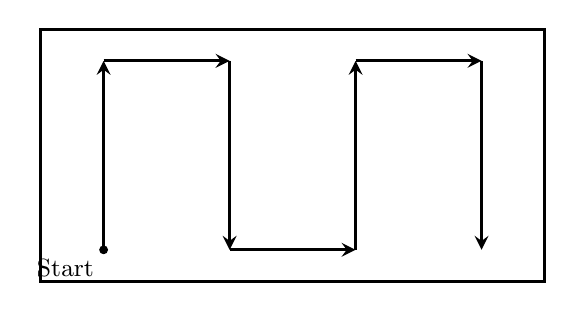
\begin{tikzpicture}[scale=0.8, >=stealth]

        % Workspace boundary
        \draw[very thick] (0,0) rectangle (8,4);



        % Connected single-pass path (one sweep per cell)
        % Cell 1
        \draw[very thick,->] (1,0.5) -- (1,3.5);
        % Move to Cell 2
        \draw[very thick,->] (1,3.5) -- (3,3.5);
        % Cell 2
        \draw[very thick,->] (3,3.5) -- (3,0.5);
        % Move to Cell 3
        \draw[very thick,->] (3,0.5) -- (5,0.5);
        % Cell 3
        \draw[very thick,->] (5,0.5) -- (5,3.5);
        % Move to Cell 4
        \draw[very thick,->] (5,3.5) -- (7,3.5);
        % Cell 4
        \draw[very thick,->] (7,3.5) -- (7,0.5);

 

        % Start marker
        \fill (1,0.5) circle (2pt);
        \node[below left] at (1,0.5) {\small Start};

    \end{tikzpicture}
    \caption{boustrophedon style coverage path.}
    \label{fig:boustrophedon}
\end{figure}




\section{Pure Pursuit Guidance}

Pure Pursuit is a geometric path-following algorithm that steers the vehicle toward a lookahead point on the desired path \cite{fossen2021handbook}. Given vehicle position $\mathbf{p} \in \mathbb{R}^2$ and path waypoints $\{\mathbf{w}_1, \ldots, \mathbf{w}_N\}$, the algorithm selects target point $\mathbf{p}_d$ at a lookahead distance along the path and computes the desired velocity:
\begin{equation}
\mathbf{v}_d = k_g \frac{\mathbf{p}_d - \mathbf{p}}{\|\mathbf{p}_d - \mathbf{p}\|}
\end{equation}
where $k_g > 0$ determines approach speed.

\section{Sliding Variables in Control}
\begin{quote}
    Hva skal jeg skrive her??? Må fine ut om definisjonen skal her eller i metode
\end{quote}
A sliding variable is a scalar or vector function that combines tracking errors with their temporal derivatives or integrals to achieve desired closed-loop dynamics \cite{slotine1991applied}. Rather than controlling each error component independently, the sliding variable formulation reduces the control problem to driving a single composite variable to zero.

For a tracking problem with position error $\mathbf{e} = \mathbf{p} - \mathbf{p}_d$, a sliding variable incorporating integral action takes the form:
\begin{equation}
\boldsymbol{\sigma} = \mathbf{e} + \lambda \int_0^t \mathbf{e}(\tau) \, d\tau
\end{equation}
where $\lambda > 0$ is a design parameter. When the sliding variable reaches zero ($\boldsymbol{\sigma} = \mathbf{0}$), the system exhibits first-order error dynamics $\dot{\mathbf{e}} = -\lambda \mathbf{e}$, ensuring exponential convergence to the desired trajectory. The integral term provides steady-state error elimination in the presence of constant disturbances, making this formulation particularly effective for systems subject to persistent external forces such as ocean currents or wind.



\section{Switching Control}

Switching control refers to feedback laws in which a plant is regulated by selecting among multiple controllers according to a discrete switching signal. Liberzon characterizes switched control systems as continuous dynamical systems whose evolution is governed by ``continuous dynamics with isolated discrete switching events'' \cite[p.~3]{liberzon2003switching}. The closed-loop system consists of several continuous subsystems,
\begin{equation}
\dot{x} = f_i(x), \qquad i \in \mathcal{M},
\end{equation}
and a switching law $\sigma(t)$ determining the active mode:  
\begin{equation}
\dot{x} = f_{\sigma(t)}(x).
\end{equation}

\subsection*{State-Dependent Switching in Continuous Systems}
Switching signals may depend on the system state. Liberzon defines this as \emph{state-dependent switching}, where transitions occur when $x(t)$ enters a region or crosses a ``switching surface'' separating the domains of different subsystems \cite[p.~5]{liberzon2003switching}. These switching surfaces partition the continuous state space, and the dynamics may switch when
\[
x(t) \in S_{ij} \;\Rightarrow\; \sigma(t^+) = j,
\]
with $S_{ij}$ denoting the boundary between subsystem $i$ and $j$.



\subsection*{Motivation for Switching Control}
Liberzon identifies specific scenarios where switching among continuous controllers is necessary \cite[p.~75]{liberzon2003switching}:
\begin{itemize}
    \item When the task inherently consists of several qualitatively different continuous behaviors, making a single feedback law unsuitable.
    \item When sensing or actuation constraints do not permit a continuous controller valid across all operating conditions.
    \item When system uncertainty or structural properties make global stabilization by a single continuous controller impossible.
\end{itemize}
Under such conditions, switching control provides a principled mechanism for achieving desired performance and stability by combining multiple continuous controllers within one hybrid closed-loop framework.

\begin{quote}
    argumenter for at dette er riktig men skal det her:::?
The system falls under all 3 categories:
1. "if the desired system trajectory is composed of entirely different types", we want to control different parameters in the moving directions, which warrants the desired behaviour of a switching controller.
2. Sensor limitations due to discrete measurements of top and bottom which is not known beforehand

Må redigere til å bare ta med matten jeg har tenkt til å bruke her
\end{quote}


\section{PID Control}
PID control provides robust control for individual degrees of freedom. For error $e(t) = r(t) - y(t)$, the control law is:
\begin{equation}
u(t) = K_p e(t) + K_i \int_0^t e(\tau) \, d\tau + K_d \dot{e}(t)
\end{equation}
where $K_p$, $K_i$, and $K_d$ provide proportional, integral, and derivative action. 

The controller can be tuned by pole placement by setting the natural frequency $\omega_{n,i}$ and damping ratio $\zeta_i$, and time constant $T_i$, the gains are:
\begin{equation}
K_{p,i} = m_i \omega_{n,i}^2, \quad K_{d,i} = 2 m_i \zeta_i \omega_{n,i} \quad K_{i,i}=K\frac{K_{p,i}}{T_{i,i}}
\end{equation}


\subsection{Anti-Windup}
Anti-windup strategies prevent integral buildup during saturation or large transients. this is an undesirable effect and can be counteracted by clamping it to a maximum, or zeroing off in new states.
´
 \chapter{Litterature review}
% \section{Background: Autonomous Net Inspection}

% Aquaculture net pens form a challenging environment for autonomous inspection. Flexible nets deform under current loads and biofouling, creating time-varying geometries that vehicles must safely navigate \cite{loland1991currentforces,lopez2015volumeloss}. Turbid water and low-light conditions limit visual sensing \cite{betancourt2020integrated}, while fish-welfare considerations restrict speed, thruster usage, and proximity to stock \cite{evjemo2024biologytech}. GPS-denied operation requires reliance on DVL, depth, attitude, and model-based navigation \cite{Amundsen2021AutonomousROV,fossen2021handbook}. Disturbances from currents and waves further impose manoeuvring limits during inspection \cite{Cardaillac2022IAS,Nguyen2024ROVControl}.

% Practical aquaculture systems therefore favour simple, robust motion patterns. Surveys show that deployed AUVs generally prioritize predictable coverage paths over computationally intensive optimisation \cite{galceran2013survey}. Representative examples include the Kalypso AUV designed specifically for cage inspection \cite{manos2024kalypso}, hybrid ROV–AUV platforms used in industrial farms \cite{papadiamantis2025hybrid}, and digital-twin validation frameworks that rely on structured trajectories \cite{scaradozzi2024digitaltwin}. These systems demonstrate a clear emphasis on repeatability, low computational load, and compatibility with limited sensor suites.

% \section{General Underwater Inspection Methods}

% \subsection{Coverage Path Planning Approaches}

% Coverage path planning typically adopts geometric patterns that guarantee completeness under uncertain localisation. Classical patterns such as boustrophedon coverage for planar surfaces \cite{choset1998coverage} and circular or cylindrical sweeps for volumetric structures \cite{lin2020planning} remain dominant. More advanced CPP approaches include bio-inspired neural networks \cite{sun2019gbnn} and field-theory-guided A* variants \cite{xu2024ftastar}, but these approaches assume sensing and computation capabilities rarely available on compact aquaculture robots.

% \subsection{Guidance Laws for Underwater Vehicles}

% Most fielded underwater robots use classical geometric guidance laws due to their robustness and low computational demand. Line-of-sight (LOS), pure pursuit, and constant bearing represent the foundational methods \cite{lekkas2009guidance,pettersen2018guidance}. Integral LOS improves disturbance rejection in currents \cite{caharija2016integral}, while pure pursuit provides a simple virtual-target formulation for path following \cite{coulter1992implementation,naeem2003pure}. When systems combine multiple inspection behaviours, the resulting hybrid architecture is naturally described using switching-system theory \cite{liberzon2003switching}.

% \section{Methods Specific to Aquaculture Net Inspection}

% \subsection{Pattern-Based Approaches for Net Cages}

% Aquaculture-specific inspection strategies commonly use cage-relative geometric patterns. DVL-based LOS guidance enables stable following of net surfaces \cite{Amundsen2021AutonomousROV}, while AUVs such as Kalypso employ cylindrical or helical paths tuned for cage geometry \cite{manos2024kalypso}. These patterns remain reliable under drift and deformation. Digital-twin studies validate such trajectories in simulation \cite{scaradozzi2024digitaltwin}. In exposed sites, disturbance-aware controllers ensure feasible manoeuvring around the cage \cite{Nguyen2024ROVControl}.

% \subsection{Perception-Centric Systems}

% Recent work emphasises perception for defect detection while using simple motion patterns. Vision-based systems integrate deep-learning hole detectors with predefined trajectories \cite{akram2023evaluating,lopezbarajas2023visualinspection,lopezbarajas2024inspection}. Sonar-driven methods similarly adopt straightforward inspection arcs aligned with sensor field of view \cite{rosa2024forwardlooking}. These approaches demonstrate the dominance of perception-centric pipelines paired with lightweight coverage strategies.

% \section{Summary and Research Gap}

% The literature consistently shows that simple geometric patterns combined with LOS or pure-pursuit guidance provide the most reliable performance for aquaculture inspection \cite{Amundsen2021AutonomousROV,manos2024kalypso}. Advanced adaptive methods exist but require dense sensing or computation unsuitable for compact, low-cost platforms \cite{xu2024ftastar}. Few works develop lightweight, geometry-based trajectories specifically tuned for cylindrical cages without relying on environmental reconstruction. This thesis addresses that gap by introducing analytically defined patterns with mode switching and an integral pure-pursuit variant that operates using only standard AUV sensors.
\section{Background: Autonomous Net Inspection}
Autonomous inspection of aquaculture net pens is shaped by flexible net structures that deform under currents and biofouling, producing continuously varying geometries \cite{loland1991currentforces,lopez2015volumeloss}. Turbid water and low-light conditions challenge camera-based sensing \cite{betancourt2020integrated}, while fish-welfare constraints restrict thruster usage and vehicle proximity to stock \cite{evjemo2024biologytech}. The lack of GPS under water makes navigation more tricky\cite{fossen2021handbook}. According to a recent report by SINTEF, there is a trend of aquaculture farms moving to more exposed areas. This leads to increased demand from autonomous inspection as the sites may be more unsafe for humans. It also increases the difficulty of motion control with increasing disturbances.\cite{SFIExposed2024}


%Practical systems need to be reliable and robust to challenging sea states. Generally \cite{galceran2013survey}. The Kalypso AUV exemplifies this trend through cylindrical cage-following patterns implemented via a fixed sequence of waypoints around the net perimeter, tuned for robustness in commercial farms \cite{manos2024kalypso}. Hybrid ROV–AUV systems combine inspection with maintenance tasks while relying on similarly predictable trajectories \cite{papadiamantis2025hybrid}. More advanced approaches, such as real-time flexible-net shape estimation and adaptive path generation from this show a promsisng direction in utilizing local measurements to gain more information\cite{amundsen2025adaptive}. This requires a model of the full pen and may not be suitable for a low cost solution. Am LLM-guided mission adaptation \cite{akram2025aquachat}, demonstrate capabilities beyond current industry norms but remain sensor- and compute-intensive.
\section{General Underwater Inspection Methods}
\subsection{Coverage Path Planning Approaches}

Generally, insepction of 3D structures utilize simple geometric paths over computationally expensive optimization mehods. Where the boustrophedon is dominating pattern for AUVs.\cite{galceran2013survey}. While advanced planners such as GBNN coverage generation \cite{sun2019gbnn} or field-theory-guided A* optimisation \cite{xu2024ftastar} offer adaptive capabilities, they depend on dense environment information, making them less suitable for low-cost aquaculture vehicles.

\subsection{Guidance Laws for Underwater Vehicles}
Most AUVs employ geometric guidance due to its reliability and low computational cost. LOS, pure pursuit, and constant-bearing methods form the classical foundation \cite{lekkas2009guidance,pettersen2018guidance}. Integral and Adaptive LOS extends this approach for improved current rejection \cite{Fossen2023ALOS, Caharija2016ILOS}. Pure pursuit, implemented via a moving virtual target \cite{coulter1992implementation,naeem2003pure}, remains effective for cable-, pipeline-, and structure-following tasks. Cardaillac and Ludvigsen propose a manoeuvring-constrained path follower, allowing heading to be fixed to the structure during inspection \cite{Cardaillac2022IAS}. 

\section{Methods Specific to net Inspection}

% \subsection{Motion-centric research}

% Net-relative geometric patterns dominate aquaculture inspection. Amundsen et al.\ employ DVL to estimate the netplane to aid the LOS-guidance law\cite{Amundsen2021AutonomousROV}. The Kalypso AUV demonstrates a net following pattern based on known geometry of the net \cite{manos2024kalypso}.Amundsen et al.\ provided an estimator for net deformation online to generate updated net-relative paths \cite{amundsen2025adaptive}. Efforts have been made to make the inspetion more efficient by empoying Hierchial task network for deciding when to inspect the net closely and from far away, but the method has yet to be tested in a real world environment \cite{lin2020planning}.


% \subsection{Perception-Centric research}
% A good portion of research toward autonomous net inspection is angled towards perception. Vision-based ROV systems integrate deep-learning hole detectors with predefined trajectories \cite{akram2023evaluating,lopezbarajas2023visualinspection}. Hybrid intervention platforms combine detection with manipulation \cite{lopezbarajas2024inspection}. Forward-looking sonar inspection uses arc-like motions aligned with the sonar field of view \cite{rosa2024forwardlooking}. LLM-mediated frameworks introduce adaptive viewpoint and segment prioritization while still relying on simple primitives \cite{akram2025aquachat}.

Research on autonomous net inspection tends to follow two complementary directions: motion-driven strategies that rely on geometric reasoning about the net, and perception-driven strategies that center sensing and interpretation. Motion-centric work primarily exploits the structure of the cage to guide vehicle behavior. Amundsen et al.\ use DVL measurements to estimate the net plane, enabling LOS guidance relative to the cage geometry \cite{Amundsen2021AutonomousROV}. Similarly, the Kalypso AUV demonstrates net-following behavior based on prior knowledge of the cage layout \cite{manos2024kalypso}. More recently, Amundsen et al.\ introduced an online estimator for net deformation, allowing continuous adaptation of planned trajectories as the structure shifts \cite{amundsen2025adaptive}. Planning efficiency has also been explored through hierarchical task networks that decide when to perform close versus coarse inspection, although this approach has yet to be validated in real-world deployments \cite{lin2020planning}.

Perception-centric research instead focuses on reliable sensing and estimation. Vision-based ROV systems integrate deep-learning hole detectors with predefined or semi-structured trajectories \cite{akram2023evaluating,lopezbarajas2023visualinspection}. Showing promising results for camera based hole detectors. In low-visibility conditions, forward-looking sonar has been used for guiding motion along the net \cite{rosa2024forwardlooking}. A research effort has proposed an LLM-based framework for increasing the autonomy in inspections by easing communication with the operator\cite{akram2025aquachat}.

\section{Summary and Research Gap}

Reliable aquaculture inspection is most commonly achieved through geometric patterns paire \cite{Amundsen2021AutonomousROV,manos2024kalypso}. Advanced adaptive planners and manoeuvring-aware control exist \cite{Cardaillac2022IAS,amundsen2025adaptive}, but their sensing and computational requirements limit deployment. There is a lack of robust inspection methods giving a full coverage guarantee. This project build upon Amundsen work on net plane and pen estimation and proposes a method which executes local net relative motion, combined with mode switching and an integral pure-pursuit variant requiring only standard AUV sensors, and aims to provide full coverage of walls.

 % 
\label{chap:Litterature}
% ===== Table + References (paste in your document body) =====

\begin{tabularx}{\textwidth}{|p{3.9cm}|p{0.6cm}|p{3cm}|p{3.5cm}|X|p{0.5cm}|}
\hline
\textbf{Article} & \textbf{Year} & \textbf{Path planning method} & \textbf{Guidance / navigation} & \textbf{Main objective} & \textbf{Ref.} \\
\hline
Planning for Fish Net Inspection with an Autonomous OSV & n/a & Hierarchical Task Network (HTN): switch between close vs. far inspection behaviors & Surface OSV with waypoint/pose tracking; vision-based hole detection & Efficient large-net inspection by balancing coverage vs. accuracy using AI mission planning & [1] \\
\hline
Research Advances in Marine Aquaculture Net-Cleaning Robots (Sensors) & 2024 & Survey of A*/APF/RRT, meta-heuristics, RL/DRL for cleaning robots & Discusses localization/SLAM and navigation strategies & Review of state-of-the-art net-cleaning robots and trends & [2] \\
\hline
Research on AUV Path Optimization Using a Field Theory-Guided A* (JMSE) & 2024 & Field-Theory-Guided A* (FT-A*); post-optimized with Dubins curves & Planner outputs waypoints; standard AUV tracking assumed & Robust 3D collision-free path planning for AUVs & [3] \\
\hline
Kalypso: an inspection AUV for aquaculture (Probe – Fishery Science \& Aquaculture) & 2024 & Simple waypoint/coverage inside cage & Vision-aided autonomous navigation; label/damage detection & Build and field-test an AUV for cage inspection & [4] \\
\hline
A systematic review on recent trends in path planning techniques for AUVs (IJIRA) & 2025 & Survey: RRT/RRT*, A*, GA/PSO, RL/DRL, hybrids & Discusses trajectory control, robustness under currents & Map recent AUV path-planning methods, challenges, gaps & [5] \\
\hline
An integrated ROV solution for underwater net-cage inspection (SN Applied Sciences) & 2020 & No explicit global planner; CV-driven inspection workflow & Operator/assisted guidance; vision-based cues & Integrate sensors and CV for net damage detection and inspection & [6] \\
\hline
Surrogate Modeling for ROV Trajectory Planning in Realistic Marine Currents (OCEANS) & 2025 & Data-assisted planning with U-Net surrogate for flow fields & Current-informed trajectory guidance (feedforward from predicted currents) & Near real-time path selection in complex currents via CFD+DL surrogate & [7] \\
\hline
Aquaculture Robotics: Adaptive Path Planning Through Real-Time Estimation of the Shape of Flexible Net Pens & 2025 & Net-pen estimator (physics-based with DVL constraints) + elastic-band path planning for net-relative waypoints & Forward-looking DVL “net-lock”; net-relative waypoint following in cylindrical coords; heading kept perpendicular to net (LOS in control stack) & Estimate full pen shape in real time and plan/follow safe, net-relative paths; validated in simulation and full-scale trials (≈0.5 m RMSE on pen shape; autonomous ROV navigation in farm) & [8] \\
\hline
Underwater ROV Software for Fish Cage Inspection (MIPRO) & 2021 & Vision-servoing-inspired following of lines/sections & ROS-based control sending depth/heading/velocity refs; visual centering & Software stack for periodic net inspection and fouling classification from video & [9] \\
\hline
A Digital Twin Infrastructure for NGC of ROV during Inspection (Robotics) & 2024 & Not a global planner; complete NGC stack within a digital twin & LOS guidance; USBL localization; PID control; co-simulation & Demonstrate full NGC + digital-twin pipeline for (semi)autonomous ROV inspection & [10] \\
\hline
Application of Maneuvering-Based Control for Autonomous Inspection of Aquaculture Net Pens (ACIRS) & 2023 & Maneuvering-based inspection trajectories (control-oriented) & Distance/heading regulation relative to cage (autonomous inspection control) & Enable autonomous net-pen inspection via maneuvering-based control & [11] \\
\hline
Automatic Visual Inspection of a Net for Fish Farms by Means of Robotic Intelligence (OCEANS) & 2023 & Trajectories controlling depth, yaw, and net distance & Vision-in-the-loop: CNN distance-to-net + feedback controller & Accurate net inspection without GPS; hole detection pipeline & [12] \\
\hline
Autonomous ROV Inspections of Aquaculture Net Pens Using DVL (preprint/manuscript) & n/a & Continuous path following along net & LOS-based nonlinear guidance using DVL-inferred local net geometry & Autonomous traverse of flexible, unknown net geometry; stability analysis & [13] \\
\hline
Complete Coverage AUVs Path Planning Based on Glasius Bio-Inspired Neural Network (GBNN) & 2019 & GBNN for single-/multi-AUV complete coverage (discrete/centralized) & Waypoint/trajectory tracking (standard AUV control) & Efficient full coverage with multi-AUV cooperation, low compute & [14] \\
\hline
Coverage Path Planning with Real-Time Replanning and Surface Reconstruction (JFR) & 2015 & Nominal path from 2.5D map + stochastic trajectory-optimization replanning & Range-based adaptation during mission & Robust 3D coverage of complex structures with onboard replanning & [15] \\
\hline
$\varepsilon^\star$: An Online Coverage Path Planning Algorithm & n/a & Online CPP via “exploratory Turing machine” + MAPS potentials & Sensor-based online navigation (unknown environments) & Guaranteed online coverage without local-extrema traps & [16] \\
\hline
Evaluating Deep Learning Assisted Automated Aquaculture Net Pens Inspection Using ROV (arXiv) & 2023 & DL-based defect detection/segmentation for inspection & On-ROV real-time detection aiding guidance & Real-time hole/debris detection in adverse conditions, embedded-ready & [17] \\
\hline
Forward-Looking Sonar Based Autonomous Aquaculture Inspection (OCEANS) & 2024 & Perimeter coverage around circular cage via circle regression & FLS-based net detection; velocity/heading refs to keep desired standoff & Circle the cage at fixed distance under low visibility & [18] \\
\hline
Inspection Operations and Hole Detection in Fish Net Cages via Hybrid Underwater Intervention System Using DL (JMSE) & 2024 & Inspection trajectories on BlueROV2 platform & CNN distance-to-net + object detection; trajectory control & End-to-end inspection/hole detection platform; tank validation & [19] \\
\hline
A Review of Path Following, Trajectory Tracking, and Formation Control for AUVs (Drones) & 2025 & Review of path following, trajectory tracking, formation control (SMC, MPC, RL, NN) & Guidance/control under uncertainty, disturbances, multi-AUV cooperation & Summarize and analyze state-of-the-art AUV guidance/control; outlook & [20] \\
\hline
An Adaptive Line-of-sight (ALOS) Guidance Law for Path Following of Aircraft and Marine Craft (TCST) & 2023 & Adaptive Line-of-Sight (ALOS) guidance; compared with ILOS and ELOS & Heading autopilot + LOS-based yaw control; disturbance compensation (drift, sideslip) & Develop and analyze ALOS for robust path following under wind/wave/current disturbances; validated on Remus 100 AUV case study & [21] \\
\hline
\end{tabularx}

\bigskip
\noindent\textbf{References}
\begin{enumerate}
  \item Lin, T.X.; Tao, Q.; Zhang, F. “Planning for Fish Net Inspection with an Autonomous OSV.” \textit{OCEANS Conference}, 2023.
  \item Liu, H.; Jiang, C.; Chen, J.; Li, H.; Chen, Y. “Research Advances in Marine Aquaculture Net-Cleaning Robots.” \textit{Sensors}, 24:7555, 2024. \url{https://doi.org/10.3390/s24237555}
  \item Xu, Z.; Shen, Y.; Xie, Z.; Liu, Y. “Research on AUV Path Optimization Using a Field Theory-Guided A* Algorithm.” \textit{JMSE}, 12:1815, 2024. \url{https://doi.org/10.3390/jmse12101815}
  \item Manos, N.; Kavallieratou, E.; Vasilopoulos, N. “Kalypso: An inspection AUV for aquaculture.” \textit{Probe – Fishery Science \& Aquaculture}, 6(1):2239, 2024. \url{https://doi.org/10.18686/fsa2239}
  \item Narayanan, V.L.; et al. “A systematic review on recent trends in path planning techniques for AUVs.” \textit{IJIRA}, 2025. \url{https://doi.org/10.1007/s41315-025-00469-9}
  \item Betancourt, J.; Coral, W.; Colorado, J. “An integrated ROV solution for underwater net-cage inspection in fish farms using computer vision.” \textit{SN Applied Sciences}, 2:1946, 2020. \url{https://doi.org/10.1007/s42452-020-03623-z}
  \item (OCEANS) “Surrogate Modeling for ROV Trajectory Planning in Realistic Marine Currents: A Methodology for Data-Assisted Underwater Navigation.” (Conference), 2025.
  \item Amundsen, H. B.; Katsidoniotaki, E.; Føre, M.; Kelasidi, E. “Aquaculture Robotics: Adaptive Path Planning Through Real-Time Estimation of the Shape of Flexible Net Pens.” \textit{IEEE Transactions on Field Robotics}, 2, 2025. \url{https://doi.org/10.1109/TFR.2025.3560245}
  \item Borković, G.; et al. “Underwater ROV Software for Fish Cage Inspection.” \textit{MIPRO}, 2021.
  \item Scaradozzi, D.; et al. “A Digital Twin Infrastructure for NGC of ROV during Inspection.” \textit{Robotics}, 13(7):96, 2024. \url{https://doi.org/10.3390/robotics13070096}
  \item Cardaillac, A.; Amundsen, H.B.; Kelasidi, E.; Ludvigsen, M. “Application of Maneuvering-Based Control for Autonomous Inspection of Aquaculture Net Pens.” \textit{ACIRS}, 2023. \url{https://doi.org/10.1109/ACIRS58671.2023.10239708}
  \item López-Barajas, S.; et al. “Automatic Visual Inspection of a Net for Fish Farms by Means of Robotic Intelligence.” \textit{OCEANS 2023}, Limerick.
  \item Amundsen, H.B.; Caharija, W.; Pettersen, K.Y. “Autonomous ROV Inspections of Aquaculture Net Pens Using DVL.” (preprint/manuscript).
  \item Sun, B.; et al. “Complete Coverage AUVs Path Planning Based on Glasius Bio-Inspired Neural Network Algorithm for Discrete and Centralized Programming.” \textit{IEEE Transactions on Cognitive and Developmental Systems}, 11(1):73–82, 2019.
  \item Galceran, E.; et al. “Coverage Path Planning with Real-Time Replanning and Surface Reconstruction for Inspection of 3D Underwater Structures.” \textit{Journal of Field Robotics}, 32(7):952–983, 2015.
  \item Song, J.; Gupta, S. “$\varepsilon^\star$: An Online Coverage Path Planning Algorithm.” (conference paper).
  \item Akram, W.; et al. “Evaluating Deep Learning Assisted Automated Aquaculture Net Pens Inspection Using ROV.” arXiv, 2023.
  \item Rosa, D.; Cabecinhas, D.; Ferreira, F. “Forward-Looking Sonar Based Autonomous Aquaculture Inspection.” \textit{OCEANS 2024 – Singapore}.
  \item López-Barajas, S.; et al. “Inspection Operations and Hole Detection in Fish Net Cages through a Hybrid Underwater Intervention System Using Deep Learning Techniques.” \textit{JMSE}, 12:80, 2024. \url{https://doi.org/10.3390/jmse12010080}
  \item He, L.; Xie, M.; Zhang, Y. “A Review of Path Following, Trajectory Tracking, and Formation Control for Autonomous Underwater Vehicles.” \textit{Drones}, 9(4):286, 2025. \url{https://doi.org/10.3390/drones9040286}
  \item Fossen, T.I. “An Adaptive Line-of-sight (ALOS) Guidance Law for Path Following of Aircraft and Marine Craft.” \textit{IEEE Transactions on Control Systems Technology}, 2023. \url{https://doi.org/10.1109/TCST.2023.3259819}
\end{enumerate}
 % 
% --- Figure ---
\begin{figure}[t]
\centering
\scalebox{0.3}{% adjust 0.9 -> 0.8 if you need it smaller
\begin{forest}
for tree={
  draw,
  rounded corners,
  align=center,
  minimum width=24mm,
  text width=26mm,
  font=\scriptsize\bfseries,
  edge={-},
  s sep=6mm,          % sibling (horizontal) separation
  l sep=6mm,          % level (vertical) separation
}
% ===== ROOT =====
[Path Planning
  % ===== Global / Graph & Geometric =====
  [Global / Graph \& Geometric
    [A* \& FT-A* \\(+ Dubins) \refn{3}]
    [D* / Variants \\(reviewed in \refn{5}]
    [Trajectory smoothing \\(post-opt)]
  ]
  % ===== Coverage (CPP) =====
  [Coverage (CPP)
    [3D CPP +\\Replanning \refn{15}]
    [Complete Coverage\\GBNN \refn{14}]
    [$\varepsilon^\star$ Online CPP \refn{16}]
  ]
  % ===== Learning / Data-driven =====
  [Learning / Data-driven
    [RL/DRL trends \\(surveys) \refn{5}]
    [Surrogate current-\\aware planning \refn{7}]
  ]
  % ===== Hybrid / Adaptive =====
  [Hybrid / Adaptive
    [Net-shape adaptive\\planner (pen est.) \refn{8}]
    [Current-aware cost\\terms in planners \refn{15}]
  ]
 ]
\end{forest}
}% end scalebox
\caption{Method map of \emph{path planning} approaches only. Superscripts refer to references [1]–[20].}
\label{fig:pathplanning-map}
\end{figure}

\chapter{System description and requirements}
 \input{inc/chapters/System}
  % ======= requirements_rov_guidance.tex (one page) =======

% --- local, tiny setup (safe to include anywhere) ---
\makeatletter
\providecommand{\REQ}{REQ}\providecommand{\NFR}{NFR}\providecommand{\SAF}{SAF}\providecommand{\INTF}{INTF}\providecommand{\ENV}{ENV}
\newcommand{\reqrow}[4]{#1 & #2 & #3 & #4\\}
\makeatother

% \section*{Requirements (Autonomous Guidance for Fish-Net Inspecting ROV)}
\small % keep it one page
\noindent\textbf{Context.} Guidance plans and drives coverage along the net surface; interfaces with nav/perception and outputs speed/heading commands to the controller.

\vspace{0.5em}
\begin{tabularx}{\textwidth}{@{}l l X l@{}}
\toprule
\textbf{ID} & \textbf{Type} & \textbf{Requirement (verifiable)} & \textbf{Verification} \\
\midrule
\reqrow{R-001}{\REQ}{Plan collision-free coverage achieving \(\ge 95\%\) net surface observed with \(\ge 20\%\) view overlap (configurable).}{Simulation}
\reqrow{R-002}{\INTF}{Output at \(\ge 5\,\mathrm{Hz}\): surge speed \(U\), heading \(\chi\), and depth \(z\).}{Test}
\reqrow{R-003}{\REQ}{Maintain standoff to net \(1\pm0.3\,\mathrm{m}\).}{Simulation}
\reqrow{R-004}{\INTF}{Accept pose \((x,y,z,\psi)\) with covariance; if \(\sigma_{xy}>1.0\,\mathrm{m}\) or DR \(>30\,\mathrm{s}\) then enter drift-safe mode (reduced speed, increased standoff).}{Simulation}
\reqrow{R-005}{\ENV}{Operate in currents up to \(0.6\,\mathrm{m/s}\); if lateral track error \(>0.5\,\mathrm{m}\) for \(>5\,\mathrm{s}\), replan or abort per safety logic.}{Simulation}
\reqrow{R-006}{\REQ}{Save areas complete and uninspected regions to database.}{Demo}
\reqrow{R-007}{\INTF}{Publish topics: \texttt{/guidance/cmd} \((U,\dot \psi,z)\), \texttt{/guidance/mode}, \texttt{/coverage/status}, \texttt{/safety/event}.}{Inspection}
\reqrow{R-008}{\NFR}{Limit required computing power to a minimum.}{Analysis/Demo}
%\reqrow{R-009}{\REQ}{Replan time for local obstacle or current change \(\le 2\,\mathrm{s}\).}{Inspection/Demo}
\reqrow{R-010}{\INTF}{Parameter set: \(U_{\max}\), rate limits, spacing to net, abort criteria.}{Analysis}
\reqrow{R-011}{\INTF}{When abort conditions are met, return to surface.}{Simulation}
\bottomrule
\label{table:req}
\end{tabularx}

\vspace{0.6em}
\noindent\textit{Verification codes:} Inspection (document/code review), Simulation (unit, test scripts).


 % \section{Line-of-Sight Guidance for Path Following}

Path following for underactuated marine vehicles such as AUVs is commonly achieved with line-of-sight (LOS) guidance laws. These algorithms generate a desired yaw angle $\psi_d$ (and optionally a desired depth $z_d$) such that the vehicle converges to and follows a straight-line path between waypoints. A large body of work has analyzed LOS-based methods, from proportional LOS \cite{fossen2003los}, integral LOS (ILOS) \cite{borhaug2008integral}, adaptive ILOS \cite{fossen2015adaptive}, and more recently, adaptive LOS (ALOS) \cite{fossen2023alos}.

\subsection{LOS Guidance Principle}
For a straight-line segment defined by two waypoints
\[
P_i^n = (x_i^n, y_i^n, z_i^n), \quad P_{i+1}^n = (x_{i+1}^n, y_{i+1}^n, z_{i+1}^n),
\]
the horizontal path azimuth is
\[
\pi_h = \atan2(y_{i+1}^n - y_i^n,\; x_{i+1}^n - x_i^n).
\]
Transforming the vehicle position $(x_n, y_n)$ into the path-tangential frame gives the cross-track error $y_e^p$:
\[
\begin{bmatrix} x_e^p \\ y_e^p \end{bmatrix}
= R_{z,\pi_h}^\top \left( \begin{bmatrix} x_n \\ y_n \end{bmatrix} - \begin{bmatrix} x_i^n \\ y_i^n \end{bmatrix} \right),
\]
where $R_{z,\pi_h}$ is a planar rotation.

\subsection{Adaptive LOS Guidance Law}
The Adaptive Line-of-Sight (ALOS) law \cite{fossen2023alos} improves robustness against ocean currents by introducing an adaptive estimate of the crab angle $\hat{\beta}_c$. The desired yaw angle is computed as
\begin{equation}
\psi_d = \pi_h - \hat{\beta}_c - \tan^{-1}\!\left(\frac{y_e^p}{\Delta_h}\right),
\label{eq:alos}
\end{equation}
with the adaptation law
\begin{equation}
\dot{\hat{\beta}}_c = \gamma_h \frac{\Delta_h}{\Delta_h^2 + (y_e^p)^2} \, y_e^p,
\label{eq:alos_update}
\end{equation}
where $\Delta_h > 0$ is the lookahead distance and $\gamma_h > 0$ is an adaptation gain.

This law guarantees uniform semiglobal exponential stability (USGES) for straight-line path following at constant speed \cite{fossen2023alos}.

\subsection{Vertical Guidance}
In this thesis, vertical control is simplified by assigning a desired depth $z_d$ directly:
\begin{equation}
z_d = z_i^n + \frac{s}{L}(z_{i+1}^n - z_i^n),
\end{equation}
where $s$ is the along-track distance in the path frame and $L$ is the horizontal path length. This avoids introducing an additional vertical LOS angle and crab compensation in heave, while still ensuring smooth depth transitions.

\subsection{Reasoning for Method Selection}
The ALOS method was chosen because:
\begin{itemize}
    \item It explicitly adapts to unknown and slowly varying sideslip/crab angles caused by ocean currents.
    \item It avoids saturation effects in ILOS, providing better transient performance when disturbances vary.
    \item It has been validated both theoretically (USGES guarantees) and experimentally on AUVs such as the Remus 100 \cite{fossen2023alos}.
    \item For the application of aquaculture net inspection, robustness against variable currents is critical, while vertical motion can be handled by a separate depth controller.
\end{itemize}

Thus, the chosen guidance structure combines ALOS in the horizontal plane with direct depth assignment in the vertical plane, ensuring robustness and practical implementability in 3D missions.

\bibliographystyle{ieeetr}
\bibliography{references}

 \part{Part 2: Guidance Methods for Planar Nets}
 \label{part:planar_guidance}
\chapter{Path Planning}

This chapter describes how the inspection path for the AUV is generated.  
The goal is to cover the entire fish net using a simple and repeatable motion pattern that guarantees full visual coverage.  The AUV will follow the path in 3D. Due to fish pen nets being a flexible structure. They are affected by currents and waves, so their exact position can not be exactly predicted. What we do know is the lenght and witch of the net. I will utilize this to make a 2D path which guarantees full coverage of the net pen. The AUV will follow in 3D. The method described below is designed to be augumented for this purpose.

\section{Reference Frame}

The path is defined in a local \textit{path frame} $\{P\}$, where:
\begin{itemize}
    \item The $z$-axis points down
    \item The $y$-axis points to the right
    
\end{itemize}

For simplicity, the path frame is currently assumed to be the same as the \textit{net frame} $\{N\}$ that follows the fish net surface, which is assumed to correspond to  \textit{North-East-Down frame} $\{NED\}$.
This means that the generated path can be used directly without additional coordinate transformations. In the future one needs to rotate the path into the netframe to follow it.

\section{Motivation}

A common and effective coverage strategy for inspection is the \textit{lawnmower} pattern.  
In this motion, the ROV moves vertically up and down while slowly progressing horizontally between each sweep.  
This pattern ensures that the entire surface is covered if the vertical and horizontal step sizes are smaller than the camera’s field of view.

\section{Analytical Path Generation}

The path is inspired by a unipolar square pulse function, which alternates between two levels.  
A MATLAB implementation of such a signal is:

\begin{lstlisting}[language=Matlab, caption={Unipolar periodic square pulse.}]
A = 10;        % Maximum amplitude
N = 10;        % Number of waves
s = linspace(0, 1, 100);
x = 100 * s;
z = (A/2) * (1 + sign(sin(2*pi*N*s)));
plot(x, z, 'LineWidth', 2);
xlabel('x [m]'); ylabel('z [m]');
title('Unipolar Periodic Square Pulse');
grid on;
\end{lstlisting}

Here, the function switches between 0 and $A$, creating a simple on–off pattern.  
The same concept is used to move the ROV up and down vertically while it gradually moves tangentially along the circumference of the net.

\section{Circular Lawn­mower Pattern in the $y$--$z$ Plane}

Let:
\begin{itemize}
    \item $R$: radius of the net,
    \item $H$: total vertical height of the inspection area,
    \item $N$: number of vertical up–down sweeps.
\end{itemize}

The path length along the net corresponds to one full circle, so the total horizontal distance in the path frame is
\begin{equation}
    W = 2\pi R.
\end{equation}

The analytical path can then be expressed as:
\begin{equation}
    z(s) = \frac{H}{2} \big( 1 + \text{sign}(\sin(2\pi N s)) \big),
\end{equation}
\begin{equation}
    y(s) = W \, s,
\end{equation}
where $s \in [0,1]$ is the path parameter.  
This gives a trajectory where the ROV moves up and down in $z$ while making a full circular sweep along the net’s circumference.

\section{Coverage and Scaling}
Because the path is described analytically, it can easily be adapted to different net sizes.  
By setting the path length equal to the circumference ($2\pi R$) and the height to the total net height $h$, the entire net can be covered.  

To guarantee full coverage, the step sizes in both the horizontal and vertical directions should be smaller than the camera’s field of view. 

\chapter{Guidance System}

This chapter describes the implementation of the guidance system, which takes the predefined path and generates reference signals for the AUV to follow the path. The algorithm operates in the two dimensional space of the yz-axis of the NED coordinate frame, All positions, velocities, and path waypoints are expressed in this frame. It outputs desired velocities in the east and down directions. In the north direction, it uses a fixed distance to the net $x_d$, which the autopilot for the surge direction controls.

The algorithm is designed to work in the simplified case where the netframe = NED, but with further extensions in mind, where the goal is to estimate the netframe relative to ned. The net will be assumed a plane, and estimated from the point cloud created by the onboard camera. For this project the plane will always be the yz-plane and the normal will be the x-axis. 

In order to avoid doing local navigation based on unaccurate estimation of global position. The path in the 2D-plane will be put into the netframe, which in the simplified case is ned, and the auv will be given references in the normal of the tangent plane. It will be recieving feedback from the perception system for when it is at the top and when it is at the bottom. It will assume it is moving with the (commanded speed or measured speed??)  along the trajectory to ensure complete coverage. once it recieves updates on top and bottom, it will update its estimate for where it is on the path by jumping to the closest path corner of the correct type. 

The vehicle is modeled as a \textbf{point mass}, and therefore only translational dynamics are considered. This is justified by the fact that the vehicle has 8 thrusters and therefor can move in all 6DOF. It is also important that the ROV moves woth the camera always facing the net, and the center of bouyancy should not be rotated to be under the center of gravity.

\section{Coordinate Frame}

We use the standard \textbf{NED} frame:
\begin{itemize}[noitemsep]
    \item $x$ – North (positive towards geographic north)
    \item $y$ – East (positive towards east)
    \item $z$ – Down (positive downward)
\end{itemize}

All positions, velocities, and path waypoints are expressed in this frame.

\section{Algorithm Overview}

Each control cycle of the \texttt{guidance\_node} executes the following steps:
\begin{enumerate}
    \item Find the K which tells us how many points ahead we need to check.
    \item Compute the distance from the current position to these points.
    \item Find the smallest distance, and select this as the next waypoint.
    \item Use this distance to compute desired velocity in y and z direction.

\end{enumerate}

\section{Mathematical Formulation}

\subsection*{Selection of Lookahead Points}
To determine how many upcoming waypoints to check, we define the number of points $k$ based on
the current vehicle speed $v$, the guidance update period $\Delta t$, and the waypoint density
$\rho$ (points per meter), and a scaling factor  $n_{\text{ahead}}$ which makes sure we check more than we need to, k will then be this number, rounded up:

\[
k = \left\lceil \rho \, v \, n_{\text{ahead}} \, \Delta t \right\rceil
\]


This ensures that the algorithm only considers the path section the vehicle can realistically reach
within the prediction horizon.


\subsection*{Nearest-Point Selection Among the Next $k$ Waypoints}

Let the index of the last accepted waypoint be $i_{\text{last}}$ and let the current
vehicle position be $P \in \mathbb{R}^3$ (NED).
Given $k$ from the lookahead rule, define the candidate waypoint set
\[
\mathcal{C} = \{\, W_{i_{\text{last}}+1},\, W_{i_{\text{last}}+2},\, \dots,\, W_{i_{\text{last}}+k} \,\}
\cap \{ W_0, \dots, W_N \}.
\]

For each candidate waypoint $W_j \in \mathcal{C}$, compute the Euclidean norm
to the current position:
\[
d_j = \| P - W_j \|, 
\qquad
j \in \bigl\{ i_{\text{last}}+1, \dots, \min(i_{\text{last}}+k,\,N) \bigr\}.
\]

Select the nearest waypoint and set the point n in front of that on the path as the next waypoint $P_d$:
\[
j^\star = \arg\min_{j \in \{ i_{\text{last}}+1,\, \dots,\, \min(i_{\text{last}}+k,\,N) \}} d_j,
\qquad
P_d = W_{j^\star + n}.
\]

If several indices $j$ give the same minimum distance, select the one with the largest index is chosen to
ensure forward progress:
\[
j^\star = \max \arg\min d_j.
\]

Finally, update the last-visited index:
\[
i_{\text{last}} \leftarrow j^\star.
\]


\subsection*{Control Objective}

We define the position error in the $yz$-plane as
\[
\mathbf{e}^p :=
\begin{bmatrix}
y \\[4pt] z
\end{bmatrix}
-
\begin{bmatrix}
y_d \\[4pt] z_d
\end{bmatrix}
=
\mathbf{p} - \mathbf{p}_d.
\]

The control objective is to drive the vehicle toward the desired point $\mathbf{p}_d$.
The desired velocity command is chosen as proportional to the normalized position error:
\[
\begin{bmatrix}
v_{E,d} \\[4pt] v_{D,d}
\end{bmatrix}
= 
-\,k _g\,
\frac{\mathbf{e^p}}{\|\mathbf{e^p}\|},
\]
where $k_g>0$ is a proportional gain determining the approach speed. This also gives the course angle in the yz plane $\chi = \text{atan2}(\omega_d, v_d)$,  

This ensures that the commanded velocity vector always points directly toward the desired position
with magnitude proportional to $k_g$.

In surge the desired distance to the net $x_d$, and the desired angle $\psi_d$ is set directly. Usually $\psi_d = 0$ and $x_d = 2\text{m}$.

\subsection*{Control Objective - with current compensation} 
We define the position error in the $yz$-plane as
\[
\mathbf{e}^p :=
\begin{bmatrix}
y \\[4pt] z
\end{bmatrix}
-
\begin{bmatrix}
y_d \\[4pt] z_d
\end{bmatrix}
=
\mathbf{p} - \mathbf{p}_d.
\]

\[
\mathbf{e}^{ct} :=
\begin{bmatrix}
y \\[4pt] z
\end{bmatrix}
-
\begin{bmatrix}
y_{j^*} \\[4pt] z_{j^*}
\end{bmatrix}
=
\mathbf{p} - \mathbf{p}_{j^*}.
\]
To compensate for current effects and unmodeled disturbances, we need to use integral effect. To acheive this introduce a sliding variabel to mimic PI-guidance law, inspired by sliding mode control.[ref]
\[ \mathbf{\sigma} = \mathbf{e^p} + \lambda \int_{0}^{\tau}{e^{ct}dt}\]
\[
\begin{bmatrix}
v_{E,d} \\[4pt] v_{D,d}
\end{bmatrix}
= 
-\,\kappa\,
\frac{\mathbf{\sigma}}{\|\mathbf{\sigma}\|},
\]
Where $\lambda$ is a tuning parameter, where 0.1 is a value which usually works well is what has showed to work well in this controller as well.
\subsection{crossing the corners}
In the case of the square path, we need to make sure that the guidance law is not cutting the corners as this will lead to strange integral effects. In addition to this, we need to make sure that integral error is not saved from segment to segment as this can lead to strange behavior as the sea state at the surface can be very different from the state at 50m depth[makes sense but have no source]. To handle these two issues, the integral state will be multiplied by the normalized values of the path normal.

To avoid the issue of incorrect behavior in the corners, the path is augumented past the corners, and the auv can only enter the next segment if it has reached the the acceptance radius of the corner

The guidance algorithm is also tested in the case of treating it as a holonomic vehicle driving in the yz-plane, and constructing the path of circle segments and straight lines. In this case the corner functionality is disabled. 
\subsection{Orientation Control Using the Surface Normal}

The vehicle’s camera must always face the net. The desired yaw and pitch follow directly
from the surface normal, which in the simplified case will be zero:

\[
\psi_d = \text{atan2}(n_{f,y},\, n_{f,x}) = 0,
\qquad
\theta_d = -\arcsin(n_{f,z}) = 0.
\]
\subsection{Current compensation}
The important factor to correct for current which moves us of track. A method to estimate the current is implemented. It updates an estimate of the current in north and east directions. As we are mostly concerned with position drift and not attitude in this case which normally is the case.
\section{Summary}

Pure Pursuit is a geometric path-following algorithm in which the vehicle continuously aims for the closest point on the path. It is a suitable choice for this application as the distances are small and the path is made up of straight lines.

By modeling the vehicle as a point pass and considering the speed in the xz directions, we keep the vehicle in the upright position. 

\chapter{ROV Dynamics and Control Laws}

\section{Kinematic and Dynamic Model}

The vehicle kinematics are expressed as
\[
\dot{\boldsymbol{\eta}} = J(\boldsymbol{\eta})\,\mathbf{v},
\]

\begin{equation}
M\dot{\boldsymbol{\nu}} + D\boldsymbol{\nu} + G(\boldsymbol{\eta}) = \boldsymbol{\tau},
\end{equation}
where
\[
M = \text{diag}(m_{11}, m_{22}, m_{33}, m_{44}, m_{55}, m_{66}), \quad
D = \text{diag}(d_{11}, d_{22}, d_{33}, d_{44}, d_{55}, d_{66}),
\]
and $G(\boldsymbol{\eta})$ contains the restoring terms in roll and pitch. Since the AUV is neutrally bouyant, one does not need to account for the g vector in the other equations.

where $\boldsymbol{\eta} = [x,\,y,\,z,\,\phi,\,\theta,\,\psi]^T$ is the generalized position in the NED frame, 
and $\boldsymbol{\nu} = [u,\,v,\,w,\,p,\,q,\,r]^T$ is the velocity vector in the body frame. The AUV is controlled by $\boldsymbol{\tau} = [\tau_1, \tau_2,\tau_3, \tau_4,\tau_5,\tau_6]$. This vector defines the forces to be applied by the thrusters computed by the control system in the 6DOF.

\section{Dynamic Equations of Motion}

Approximating the AUV model as a decoupled mass-damper-spring systems. This is a good assumption because we are moving slowly, which means we will have weak coupling between the hydrodynamic coefficients in the degress of freedom, and the linear damping terms will dominate over the quadratic ones. We are also operating in the upright position, with small angles in roll and pitch. the 6-DOF dynamic equations for the AUV are
\begin{align*}
m_{11}\dot{u} + d_{11}u &= \tau_1, \\[4pt]
m_{22}\dot{v} + d_{22}v &= \tau_2, \\[4pt]
m_{33}\dot{w} + d_{33}w &= \tau_3, \\[4pt]
m_{44}\dot{p} + d_{44}p + W(z_g - z_b)\phi &= \tau_4, \\[4pt]
m_{55}\dot{q} + d_{55}q + W(z_g - z_b)\theta &= \tau_5, \\[4pt]
m_{66}\dot{r} + d_{66}r &= \tau_6,
\end{align*}
where $m_{ii}$ are the rigid body and added mass terms, $d_{ii}$ are the linear damping coefficients,
and $W= mg$ represents the weight. 

\subsection*{Transformation from NED to Body Frame}

The guidance node provides desired velocities in the NED frame for motion
along the net surface, i.e.\ in the east--down plane:
\[
\mathbf{v}_d^n =
\begin{bmatrix}
v_{E,d} \\[4pt]
v_{D,d}
\end{bmatrix}.
\]
The ROV controller, however, operates in the body-fixed frame, where the corresponding
velocities are the sway and heave components,
\[
\mathbf{v}_d^b =
\begin{bmatrix}
v_d \\[4pt]
w_d
\end{bmatrix}.
\]

The transformation between the two is obtained from the vehicle's yaw-angle~$\psi$,
assuming small roll and pitch angles ($\phi,\theta \approx 0$):
\[
\mathbf{v}_d^b = R_{n,2D}^b(\psi)\,\mathbf{v}_d^n,
\qquad
R_{n,2D}^b(\psi) =
\begin{bmatrix}
\cos\psi & 0 \\[4pt]
0 & 1
\end{bmatrix}.
\]
However, since the AUV moves primarily along the net (east--down directions)
and the surge axis is used for distance control, the rotation is simplified
to include only the vertical component:
\[
\begin{bmatrix}
v_d \\[4pt] w_d
\end{bmatrix}
=
\begin{bmatrix}
v_{E,d} \\[4pt] v_{D,d}
\end{bmatrix}.
\]


These are then used as inputs to the corresponding control laws.

\subsection*{Control Laws}
We let the body $x$-axis point toward the net. The primary task in surge is therefore
to regulate the distance to the net to zero. This is done with a position–damping
controller in surge, while sway and heave are controlled in velocity.

\begin{align}
\tau_1 &= -K_{p_1}\,(x - x_d) - K_{d_1}\,u + K_{i_1}*e_{int}, \label{eq:surge-net}\\[4pt]
\tau_2 &= -K_{p_2}\,(v - v_d) \label{eq:sway-vel}\\[4pt]
\tau_3 &= -K_{p_3}\,(w - w_d) \label{eq:heave-vel}\\[4pt]
\tau_4 &= 0, \\[4pt]
\tau_5 &= 0, \\[4pt]
\tau_6 &= -K_{p_6}\,(\psi - \psi_d) - K_{d_6}\,r - K_{i_6}\psi_{int}. \label{eq:yaw}
\end{align}

Here $x$ is the measured distance to the net expressed in the surge direction, this distance is expressed in NED frame.
The term $-K_{d_1}u$ provides damping in surge to avoid collision with the net.
The sway and heave channels, track body-frame velocity commands $(v_d, w_d)$ delivered by the guidance node, enabling motion along and up/down the net while the surge controller maintains the distance. The $\psi_d$ is provided by the guidance node, also in the simplified case set to zero.

\subsection{Controller Tuning}

The proportional and derivative gains are selected based on the decoupled second-order mass--damper--spring model for each degree of freedom. 
For the surge and yaw axes, the dynamics are described by
\begin{equation}
    m_i \dot{v}_i + d_i v_i = \tau_i,
\end{equation}
with a PD control law
\begin{equation}
    \tau_i = -K_{p_i}(v_i - v_{d_i}) - K_{d_i}v_i.
\end{equation}
The resulting closed-loop dynamics yield
\begin{equation}
    m_i \dot{v}_i + (d_i + K_{d_i})v_i + K_{p_i}(v_i - v_{d_i}) = 0,
\end{equation}
which corresponds to a second-order system with
\begin{equation}
    \omega_{n_i} = \sqrt{\frac{K_{p_i}}{m_i}}, \qquad 
    \zeta_i = \frac{d_i + K_{d_i}}{2\sqrt{m_i K_{p_i}}}.
\end{equation}
The gains can thus be chosen as
\begin{equation}
    K_{p_i} = m_i \omega_{n_i}^2, \qquad 
    K_{d_i} = 2 m_i \zeta_i \omega_{n_i} - d_i.
\end{equation}

For sway and heave, only velocity control is required. 
The control input is therefore simplified to
\begin{equation}
    \tau_i = -K_{d_i}(v_i - v_{d_i}),
\end{equation}
leading to the first-order closed-loop dynamics
\begin{equation}
    m_i \dot{v}_i + (d_i + K_{d_i})v_i = K_{d_i}v_{d_i},
\end{equation}
with time constant
\begin{equation}
    T_i = \frac{m_i}{d_i + K_{d_i}}.
\end{equation}
For roll and pitch, the restoring moments $W(z_g - z_b)\phi$ and $W(z_g - z_b)\theta$ stabilize the vehicle around zero angles, and no active control ($\tau_4 = \tau_5 = 0$) is required.



\section{Summary}

The equations above define a decoupled 6-DOF AUV model with independent control
laws for surge, sway, heave, and yaw.
For roll and pitch, the restoring terms naturally stabilize the vehicle around
zero angles, and no active control ($\tau_4 = \tau_5 = 0$) is required.


\chapter{Mode Controller}

This chapter describes the implementation of the mode based guidance and control, which executes the coverage pattern along the net by switching between a discrete set of motion commands. Unlike the guidance system, which computes geometric references based on path waypoints, the mode controller defines the \emph{operational logic} describing the path. 

The mode controller outputs surge, sway, heave, and yaw force commands directly from a set of PID and P control laws. These control actions ensure that the AUV maintains a constant standoff distance to the net, moves with a predefined scanning velocity, and transitions cleanly at top and bottom corners without accumulating unwanted integral error.

The controller assumes that the vehicle can be modeled as a point mass due to its 8-thruster configuration. For all operational modes, the ROV must maintain its camera pointing toward the net, and the vehicle should remain upright to avoid undesirable shifts in the relationship between the center of mass and center of buoyancy.

\section{Coordinate Frames and Motion Modes}

All states are expressed in the standard \textbf{NED} frame:
\begin{itemize}[noitemsep]
    \item $x$ – North (positive toward the net normal)
    \item $y$ – East (horizontal direction along the net)
    \item $z$ – Down (vertical direction along the net)
\end{itemize}

The mode controller operates on four discrete motion modes:
\begin{enumerate}
    \item Mode 0: Vertical descent along the net
    \item Mode 1: Vertical ascent along the net
    \item Mode 2: Horizontal motion at the bottom edge
    \item Mode 3: Horizontal motion at the top edge
\end{enumerate}

Each mode defines which axis is performing tracking, which is holding depth, and which velocities are treated as feedforward references.

\section{Initialization}

On first activation, the controller initializes:
\begin{itemize}[noitemsep]
    \item Net boundaries: $z_{\text{top}} = 0$, $z_{\text{bot}} = H$
    \item Vertical mode: \texttt{mode\_z} = \texttt{0} (descending)
    \item Horizontal reference: $y_d = 0$
    \item Standoff distance: $x_d = 2\,\mathrm{m}$
    \item Nominal actuation velocities: $w_d = 1\,\mathrm{m/s}$ (vertical), $v_d = 1\,\mathrm{m/s}$ (horizontal)
    \item All integral terms set to zero
\end{itemize}

\section{Mode Logic}

At each control cycle, the controller selects forces $\tau = [\tau_1,\dots,\tau_6]^T$ corresponding to surge, sway, heave, roll, pitch, and yaw.

\subsection{Vertical Descent (Mode 0)}

The vehicle moves downward with desired velocity $w_d$, while regulating sway position to remain aligned with the column:

\[
\tau_2 = 
- K_{p2}(y - y_d) 
- K_{d2} v 
- K_{i2} \int (y - y_d)\,dt
\]

To ensure smooth transitions into the bottom corner, the reference vertical speed is reduced in the last few decimeters:

\[
w_{\text{ref}} = \max \left( w_{\min},\, \alpha w_d \right),
\qquad 
\alpha = \min\left(1,\frac{|z - z_{\text{bot}}|}{d_{\text{corner}}}\right)
\]

\[
\tau_3 = -K_{p3}(w - w_{\text{ref}})
\]

When $|z - z_{\text{bot}}| < 0.2$, the controller switches to Mode~2 (horizontal motion along the bottom).

\subsection{Vertical Ascent (Mode 1)}

Similar logic applies for ascending the net:

\[
w_{\text{ref}} = -\max \left( w_{\min},\, \alpha w_d \right)
\]

When $|z - z_{\text{top}}| < 0.2$, the controller switches to Mode~3.

\subsection{Horizontal Motion Along the Bottom (Mode 2)}

The controller tracks a constant sway velocity toward the next vertical scanline:

\[
v_{\text{ref}} = \max\left(v_{\min},\, \alpha v_d\right),
\qquad 
\alpha = \min\left(1, \frac{|(y_d + SW) - y|}{d_{\text{corner}}}\right)
\]

\[
\tau_2 = -K_{p2}(v - v_{\text{ref}})
\]

Depth is held at $z = z_{\text{bot}}$ using a full PID law:
\[
\tau_3 = -K_{p3}(z - z_d) - K_{d3}w - K_{i3}\int(z - z_d)\, dt
\]

When $y = y_d + SW$ (within $0.2\,\mathrm{m}$), the controller switches to Mode~1.

\subsection{Horizontal Motion Along the Top (Mode 3)}

Identical to Mode~2 but maintaining depth at $z_{\text{top}}$ and transitioning into descent at the next vertical boundary.

\section{Surge, Roll, Pitch, and Yaw Control}

\subsection{Surge (Standoff Regulation)}
The standoff distance to the net is maintained by:

\[
\tau_1 = 
- K_{p1}(x - x_d) 
- K_{d1} u 
- K_{i1} \int(x - x_d)\,dt
\]

\subsection{Roll and Pitch}

Since the ROV must remain upright:

\[
\tau_4 = 0, \qquad \tau_5 = 0
\]

\subsection{Yaw Control}

Yaw is regulated to maintain the camera normal aligned with the net: 

\[
\psi_{\text{err}} = \text{ssa}(\psi - \psi_d)
\]

\[
\tau_6 = 
- K_{p6} \psi_{\text{err}}
- K_{d6} r
- K_{i6} \int \psi_{\text{err}}\,dt
\]

\section{Integral Handling and Corner Behavior}

To avoid unbounded integral buildup due to the sharp geometric transitions at corners:
\begin{itemize}
    \item Integral terms for $y$ and $z$ are reset at each mode transition.
    \item Corner slowdown ensures that the PID loops do not experience abrupt sign changes.
    \item Horizontal and vertical integral actions are never carried across segments.
\end{itemize}

This ensures stable behavior even when vertical current varies significantly between surface and depth.




\part{Part 3: Guidance Method for Cylindrical Nets}
\label{part:cylindrical_guidance}
\chapter{Mode Based Cylindrical Sweep Inspection Controller}

This chapter presents the augmentation from planar nets aligned with NED, to inspection of a deformed cylindrical fish-net. The vehicle follows a lawnmower pattern defined on the net surface while maintaining a constant clearance from the net and aligning its attitude with the net normal. inspired by \cite{Amundsen2021AutonomousROV}\cite{Amundsen2024AquacultureRobotics} \cite{Cardaillac2022IAS}

\section{State Inputs and Geometry Quantities}

At each control step, the controller receives:
\begin{itemize}
    \item Vehicle pose:
    \[
        \eta = 
        \begin{bmatrix}
            x & y & z & \phi & \theta & \psi
        \end{bmatrix}^\top ,
    \]
    \item Body–fixed velocities:
    \[
        \nu =
        \begin{bmatrix}
            u & v & w & p & q & r
        \end{bmatrix}^\top ,
    \]
    \item Cylinder geometry information at the vehicle position:
    \begin{itemize}
        \item $\theta_{\mathrm{rel}}$: angle around the cylinder, where it is assumed the estimation is able to estimate net deformation and movement.
        \item $n_{\mathrm{net}} \in \mathbb{R}^3$: \emph{inward} surface normal of the net.
        \item $s_{\mathrm{clear}}$: clearance to the net along the inward normal:
    \end{itemize}
\end{itemize}

The pattern–following logic maintains:
\begin{itemize}
    \item the current stripe angle $\theta_k$,  
    \item the next stripe angle $\theta_{k+1} = \theta_k + \Delta\theta$,
\end{itemize}
with $\Delta\theta$ defined by the field of view of the camera.

\section{Control Output}

The controller computes the generalized force vector
\[
    \tau = 
    \begin{bmatrix}
        \tau_1 & \tau_2 & \tau_3 & \tau_4 & \tau_5 & \tau_6
    \end{bmatrix}^\top ,
\]
corresponding to body–fixed surge, sway, heave, roll, pitch, and yaw.
All controllers are a form of P, and PID controllers.

\section{Surge Control: Controlling distance to the Net}

The vehicle must remain keep a set distance to the net to allow the camera to see the net, and avoid collsions with the net, this distance is $x_d$. The inward clearance error is
\[
    e_s = \text{distNet} - x_d .
\]

A PID regulator is applied in the surge direction:
\begin{align}
    \tau_1
    &= -K_{p1} e_s - K_{d1} u - K_{i1} \int e_s \, dt .
\end{align}

Since the vehicle's body $x$–axis, this control law ensures that
\[
    \text{distNet} \to x_d \qquad .
\]

\section{Planar Sway and Heave Control}

The planar motion controllers regulate the vehicle either:
\begin{enumerate}
    \item vertically along a stripe ($\theta \approx \theta_k$), or
    \item horizontally along the top or bottom edge 
          ($\theta \to \theta_{k+1}$).
\end{enumerate}

\subsection{Stripe Tracking (Vertical Legs)}

When moving vertically, angle around the net is performed using:
\[
    e_\theta = \operatorname{ssa}\!\left(\theta_{\mathrm{rel}} - \theta_k\right),
\]
with sway control
\[
    \tau_2 = 
        -K_{p\theta} e_\theta 
        - K_{d\theta} v
        - K_{i\theta} \int e_\theta \, dt .
\]

Vertical speed is controlled by a PD law with a depth–dependent reference
\[
    w_{\mathrm{ref}} = 
    \begin{cases}
        \;\;\; w_d \, \alpha(z), & \text{descending},\\[2mm]
        - w_d \, \alpha(z), & \text{ascending},
    \end{cases}
\]
where $\alpha(z) \in [0,1]$ is a slowdown factor near the top/bottom.

Heave control:
\[
    \tau_3 = -K_{p3}(w - w_{\mathrm{ref}}).
\]

\subsection{Horizontal Motion (Bottom/Top Legs)}

When sweeping horizontally between adjacent stripes,
the angle error to the next stripe is
\[
    e_{\theta,\mathrm{next}} =
    \operatorname{wrap}\!\left(\theta_{\mathrm{rel}} - \theta_{k+1}\right).
\]

Sway control drives the vehicle toward $\theta_{k+1}$:
\[
    \tau_2 = - K_{d\theta} (v_d -v).
\]

Depth regulation keeps the vehicle at the top or bottom boundary:
\[
    \tau_3 = 
        -K_{p3z}(z - z_d)
        -K_{d3} w
        -K_{i3} \int (z - z_d)\, dt .
\]

When the condition
\[
    |e_{\theta,\mathrm{next}}| < \varepsilon_\theta
\]
is met, the controller advances the pattern:
\[
    \theta_k \leftarrow \theta_{k+1}, \qquad
    \theta_{k+1} \leftarrow \theta_k + \Delta\theta .
\]

\section{Attitude Control and Net Alignment}\label{sec:attitude}

The inward surface normal is denoted $n_{\mathrm{net}} = [n_x, n_y, n_z]^\top$.
We align the body $x$–axis with this normal using pitch and yaw commands.

A 3–2–1 (yaw–pitch–roll) orientation gives the forward axis:
\[
    a_x =
    \begin{bmatrix}
        \cos\theta \cos\psi \\[2mm]
        \cos\theta \sin\psi \\[2mm]
        -\sin\theta
    \end{bmatrix}.
\]

We desire:
\[
    a_x^{\,d} = n_{\mathrm{net}} .
\]

From the forward–axis equations, the desired pitch and yaw satisfy:
\begin{align}
\theta_d &= \operatorname{atan2}\!\left(-n_z,\, \sqrt{n_x^2 + n_y^2}\right), &
\psi_d &= \operatorname{atan2}(n_y, n_x).
\end{align}

Yaw and pitch errors:
\[
    e_\theta^{\mathrm{att}} = \theta - \theta_d, \qquad
    e_\psi^{\mathrm{att}}   = \psi - \psi_d.
\]

Pitch control:
\[
    \tau_5 =
        -K_{p5} e_\theta^{\mathrm{att}}
        -K_{d5} q
        -K_{i5} \int e_\theta^{\mathrm{att}} dt .
\]

Yaw control:
\[
    \tau_6 =
        -K_{p6} e_\psi^{\mathrm{att}}
        -K_{d6} r
        -K_{i6} \int e_\psi^{\mathrm{att}} dt .
\]

Roll stabilization maintains $\phi \approx 0$:
\[
    \tau_4 = -K_{p4} \phi - K_{d4} p.
\]

\section{Summary of Full Control Law}

The total generalized force vector is
\[
    \tau =
    \begin{bmatrix}
        \tau_1 \\ \tau_2 \\ \tau_3 \\ \tau_4 \\ \tau_5 \\ \tau_6
    \end{bmatrix}.
\]

Each element comes from physically–motivated control objectives:
\begin{itemize}
    \item $\tau_1$: regulate inward clearance from the net,
    \item $\tau_2$: keep constant angle in net, and control speed during horizontal movement  to next stripe.
    \item $\tau_3$: keep constant heave during horizontal movement, and control speed during vertical movement.
    \item $\tau_4$: roll stabilization.
    \item $\tau_5$: pitch alignment with net normal.
    \item $\tau_6$: yaw alignment with net normal.
\end{itemize}

This produces a control law able to follow the net and its deformations.

% 

\chapter{Mode-Based Net-Following Control} In this chapter we present and analyze a mode-based hybrid controller used for autonomous inspection of cylindrical aquaculture nets using an underwater vehicle (AUV/ROV). The controller organizes the motion into four modes: moving \emph{down} along a vertical stripe, \emph{up} along a vertical stripe, \emph{bottom horizontal} motion, and \emph{top horizontal} motion. Together these modes generate a systematic ``lawnmower''-like pattern around the net. We prove fundamental properties about the stability of the closed-loop behavior and justify the switching logic. 
\section{Controller Overview} Let ``$\eta = (x,y,z,\phi,\theta,\psi)$'' denote the pose in earth-fixed coordinates and Euler angles, and let ``$\nu = (u,v,w,p,q,r)$'' denote the body velocity vector. The control input is the generalized force vector ``$\tau = (\tau_1,...,\tau_6)$``. The net surface is parameterized by an inward-pointing surface normal ``$n_\mathrm{net}$`` and a scalar ``$s_\mathrm{clear}$`` describing the signed clearance along this normal, where positive means the vehicle is inside, zero means exactly on the net, and negative means outside. The controller uses persistent internal state variables to represent the current stripe angle, the next stripe angle, vertical mode logic, and integral terms used for PI control in several channels. The mode variable is an integer ``$m \in \{0,1,2,3\}$`` with the meaning: \begin{itemize} \item $m=0$: vertical motion down along stripe $\theta=\theta_\mathrm{curr}$, \item $m=1$: vertical motion up, \item $m=2$: horizontal motion along the bottom toward $\theta_\mathrm{next}$, \item $m=3$: horizontal motion along the top. \end{itemize} Each mode implements a feedback law that is smooth within the mode. Switching occurs when the AUV reaches the bottom, top, or the next stripe angle.
\section{Surge-Clearance Control} The first DOF regulates the inward clearance:\[ s_\mathrm{clear} \to x_d, \] where $x_d>0$ is the desired inward offset from the net. A PI controller with velocity damping is applied: \begin{equation} \tau_1 = -K_{p1}( s_\mathrm{clear} - x_d ) - K_{d1} u - K_{i1} \, \int (s_\mathrm{clear}-x_d)\,dt. \end{equation} This is a standard exponentially stabilizing PD--PI controller for regulating a scalar reference under bounded disturbances. Under the assumption that the surge dynamics are input-signal strictly passive (standard for underwater vehicles), the closed loop is input-to-state stable (ISS). The integral term ensures zero steady-state error. 
\section{Sway Angle Tracking in Vertical Modes} When moving vertically ($m=0$ or $m=1$), the controller attempts to keep the vehicle aligned with the stripe described by angle $\theta_\mathrm{curr}$. Define the stripe tracking error \begin{equation} e_\theta = \operatorname{ssa}(\theta_\mathrm{rel} - \theta_\mathrm{curr}), \end{equation} where $\operatorname{ssa}(\cdot)$ wraps angles to $(-\pi,\pi]$. The sway controller is \begin{equation} \tau_2 = -K_{p\theta} e_\theta - K_{d\theta} v - K_{i\theta} \int e_\theta \,dt. \end{equation} Again, under standard marine-vehicle passivity assumptions, this is a globally stable PI-damped controller with exponential convergence of $e_\theta$. 
\section{Vertical Velocity Control and Corner Slowdown} To move vertically with nominal rate $w_d$, the controller applies \begin{equation} \tau_3 = -K_{p3}(w - w_\mathrm{ref}), \end{equation} where the reference $w_\mathrm{ref}$ is filtered near the top/bottom boundaries with a corner slowdown factor \begin{equation} w_\mathrm{ref} = \operatorname{sign}(\text{direction}) \cdot \max( w_\mathrm{corner,min},\; w_d \, \alpha ),\quad \alpha = \min\left(1, \frac{\mathrm{dist}}{d_\mathrm{corner}}\right). \end{equation}  This ensures smooth deceleration before switching modes, avoiding Zeno behavior. The resulting subsystem is an overdamped first-order system that guarantees boundedness and smoothness. 

\section{Horizontal Modes and Stripe Updates} In bottom and top horizontal modes ($m=2,3$), the system moves tangentially around the net at desired_velocity $v_d$ using the sway controller \begin{equation} \tau_2 = -K_{p\theta}(v - v_d). \end{equation} Depth is maintained by a PI controller: \begin{equation} \tau_3 = -K_{p3,z}(z - z_d) - K_{d3} w - K_{i3} \int (z - z_d) \, dt. \end{equation} The next stripe angle $\theta_{\text{next}}$ is reached once ``$\theta_{\mathrm{rel}} > \theta_{\mathrm{next}} - \theta_{\mathrm{tol}}$``. Because $\theta_\mathrm{rel}$ is monotonic in the horizontal traversal, the condition is well-posed. Switching is thus deterministic and nonambiguous. \section{Attitude Alignment with the Net Surface} The desired body $x$-axis direction is the inward surface normal $n$. Using ZYX Euler angles, the direction of the body $x$-axis is \begin{equation} d(\phi,\theta,\psi) = (\cos\theta\cos\psi,~ \cos\theta\sin\psi,~ -\sin\theta). \end{equation} Equating $d=n$ yields desired attitudes \begin{equation} \theta_d = -\arcsin(n_z), \qquad \psi_d = \operatorname{atan2}(n_y,n_x). \end{equation} Errors are \begin{equation} e_\theta = \operatorname{ssa}(\theta-\theta_d), \qquad e_\psi = \operatorname{ssa}(\psi-\psi_d). \end{equation} The pitch and yaw controllers are \begin{align} \tau_5 &= -K_{p5} e_\theta - K_{d5} q - K_{i5}\!\int e_\theta dt,\\ \tau_6 &= -K_{p6} e_\psi - K_{d6} r - K_{i6}\!\int e_\psi dt. \end{align} The roll axis is damped to 0 using \begin{equation} \tau_4 = -K_{p4} \phi - K_{d4} p. \end{equation} Because the attitude dynamics are passive and the reference is constant in each mode, these PI-damped controllers guarantee exponential convergence modulo the Euler singularity set, which is never reached due to the physical geometry of a net. \section{Closed-Loop Hybrid Stability} The full system is a hybrid automaton with four continuous domains and three switching surfaces. Each continuous domain has a smooth control Lyapunov function (CLF): a weighted sum of squared tracking errors in\ $s_\mathrm{clear}$, $z$, tangential $v$, attitude errors, and integral states. At switching events, the CLF does not increase because: \begin{enumerate} \item Stripe updates reset only the stripe-integral state, which eliminates stored energy. \item Vertical transitions occur at physical boundaries ($z=0$ or $z=H$) where vertical velocity is already near zero due to corner slowdown. \item Other states ($u,v,p,q,r$) are continuous. \end{enumerate} Thus the hybrid system satisfies the standard dwell-time condition and has no Zeno executions. The CLF decreases strictly in each mode, hence the system is globally asymptotically stable with respect to the desired stripe-following orbit. \section{Conclusion} We have presented a complete description of the mode-based controller used for net inspection. Each mode is individually stable and smooth, while switching is triggered by geometric events that preserve Lyapunov stability. The resulting hybrid closed-loop system produces a predictable, robust stripe pattern that fully covers the net and maintains safe clearance, alignment, and depth. 
\end{verbatim}

 \chapter{illustration}
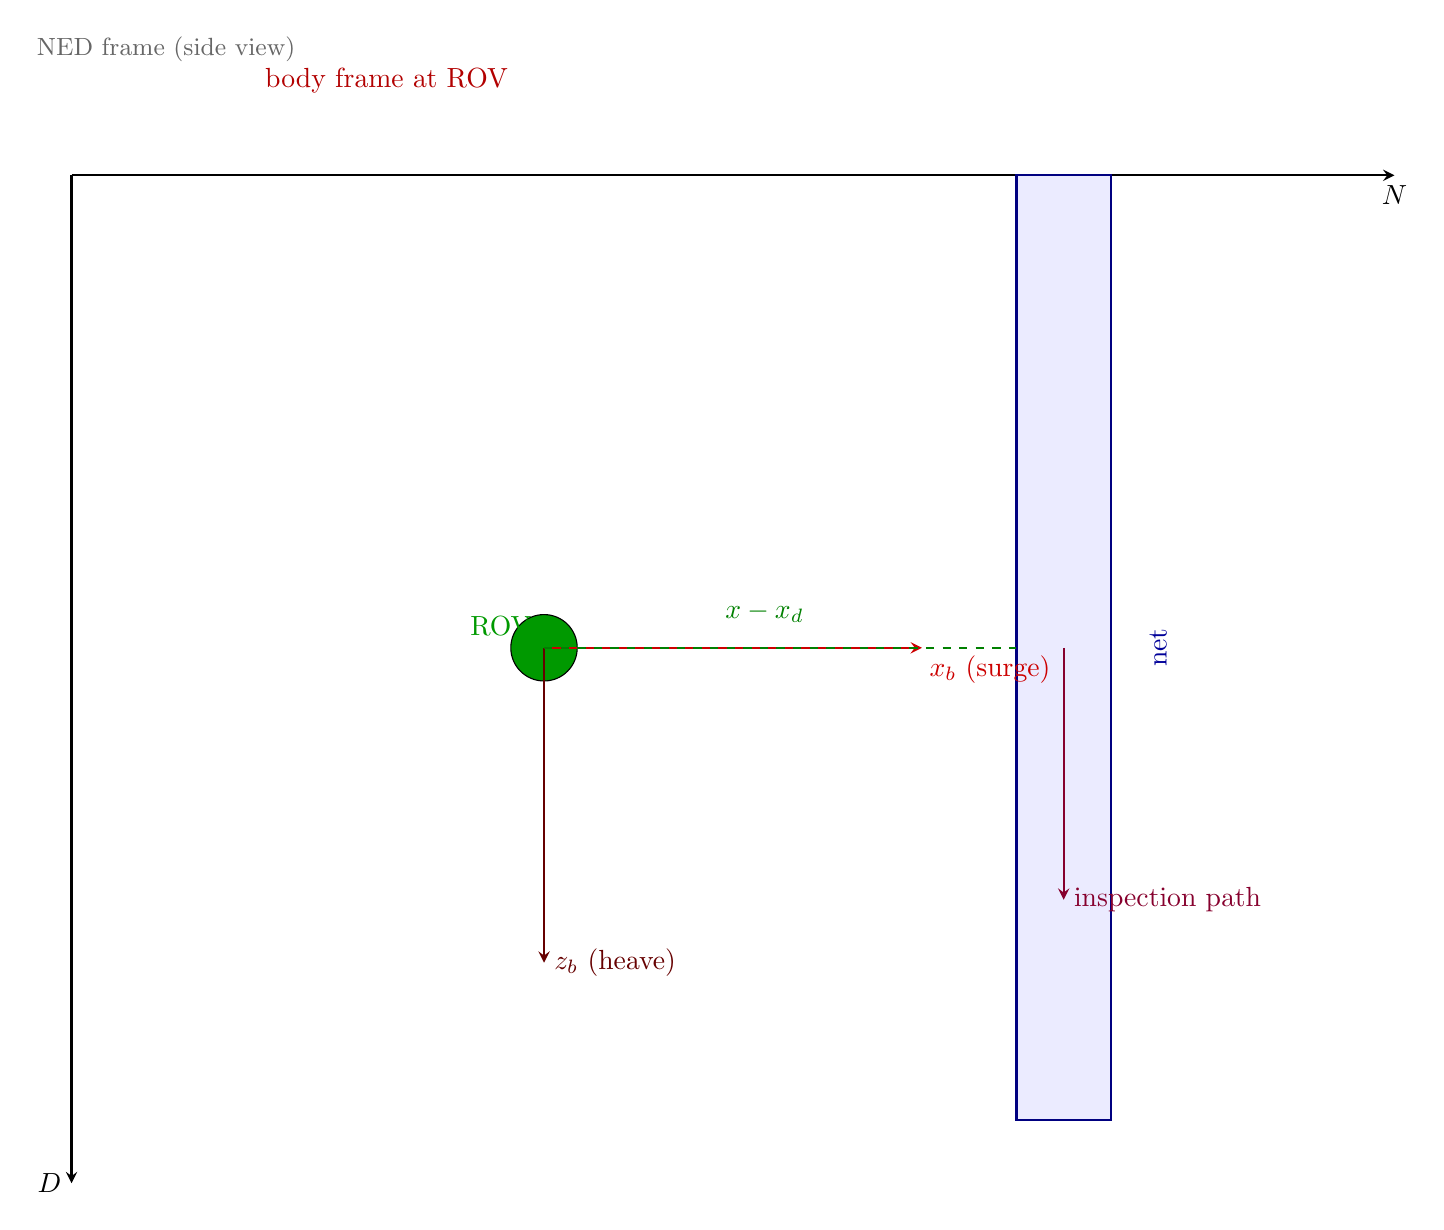
\begin{tikzpicture}[scale=4.0,>=stealth]

  %--- NED axes (N horizontal, D down) ---
  \draw[->,thick] (0,0) -- (4.2,0) node[below] {$N$};
  \draw[->,thick] (0,0) -- (0,-3.2) node[left] {$D$};
  \node[black!60] at (0.3,0.4) {\small NED frame (side view)};

  %--- Net plane ---
  \draw[fill=blue!8,draw=blue!50!black,thick]
        (3,0) -- (3,-3) -- (3.3,-3) -- (3.3,0) -- cycle;
  \node[blue!60!black,rotate=90] at (3.45,-1.5) {net};

  %--- ROV position ---
  \coordinate (rov) at (1.5,-1.5);
  \draw[fill=green!60!black] (rov) circle (3pt);
  \node[green!60!black,above left=1pt] at (rov) {ROV};

  %--- Body axes (x_b forward to net, z_b down) ---
  \draw[->,red!80!black,thick] (rov) -- ++(1.2,0)
      node[below right=-1pt] {$x_b$ (surge)};
  \draw[->,red!40!black,thick] (rov) -- ++(0,-1.0)
      node[right] {$z_b$ (heave)};

  %--- Distance to net (along body x) ---
  \draw[dashed,green!50!black,thick] (rov) -- (3,-1.5);
  \node[green!50!black,above] at (2.2,-1.45) {$x - x_d$};

  %--- Inspection motion along the net (up/down) ---
  \draw[->,purple!70!black,thick] (3.15,-1.5) -- ++(0,-0.8)
      node[right] {inspection path};

  %--- Annotate body frame ---
  \node[red!70!black] at (1.0,0.3) {body frame at ROV};

\end{tikzpicture}
 \chapter{Simulation and Tests}

This chapter describes how the developed guidance and control framework was tested in simulation. The objective was to verify that the system meets the functional requirements defined in Chapter~1, 
including coverage, stability, and safety under loss of localization and external disturbances.

\section{Simulation Setup}

The system was executed in a closed-loop configuration consisting of the following modules:
\begin{itemize}
    \item \texttt{path planner}: Generates the lawnmower pattern in 2D.
    \item \texttt{path manager}: chooses the next waypoint and stores observed and unobserved regions
    \item \texttt{Pure pursuit}: Implements the Pure Pursuit algorithm and outputs desired velocities $(v_{E,d}, v_{D,d})$.
    \item \texttt{autopilot}: Applies the control laws described in Chapter~5 to compute thrust forces.
    \item \texttt{simulator}: Integrates the dynamic equations and publishes position and orientation.
\end{itemize}

Each simulation used a timestep of $\Delta t = 0.05~\text{s}$ for the control loop and $\Delta t_g = 0.1~\text{s}$ for the guidance update.
The cylindrical fish pen was modeled with radius $R = 12~\text{m}$ and height $H = 20~\text{m}$.
The nominal standoff distance to the net was $x_d = 2.0~\text{m}$, and the ROV was assumed to cover 4m with each sweep

At each guidance step $k$, the position estimate was obtained
\[
\eta_k = [x_k, y_k, z_k, \psi_k]^T, \qquad 

\]
The position was propagated by Euler integration of the dynamic model:
\begin{equation}
\eta_{k+1} = \eta_k + \dot{\eta}_k \Delta t, \qquad \dot{\eta}_k = J(\eta_k)\nu_k.
\end{equation}

\section{Guidance Execution}

At each control cycle, the Pure Pursuit algorithm determined the next reference point $p_d$ on the path:
\begin{equation}
j^\star = \arg\min_{j \in \{i_{\text{last}}+1, \dots, i_{\text{last}}+k\}} 
\| P_k - W_j \|, \qquad
p_d = W_{j^\star + n}.
\end{equation}
The desired velocity in the $y$--$z$ plane was then computed as
\begin{equation}
\nu_{d,k} = -k_g \frac{(p_k - p_{d,k})}{\|p_k - p_{d,k}\|}.
\end{equation}

The controller received these references and generated thrust commands in surge, sway, heave, and yaw, 
ensuring stable motion along the net surface.

\section{Loss of Position}

The system does not perform estimation itself, but relies on external navigation module. When this fails to provide a position, it will integrate its own position based on desired velocities. It will continue along path for 1s, after 2s the system enter a \textit{drift-safe mode}, defined as
\begin{equation}
U_d \leftarrow 0.5U_d, \qquad x_d \leftarrow x_d + 1~\text{m}.
\end{equation}
This reduced the surge velocity and increased the standoff distance to prevent collision with the net. If position returned normal operations preceded. After running in drift safe mode for 10s it will abort the mission.

\section{Loss of distance to net}

treated same as loss of position, enter drift safe mode




\section{Current Disturbance}

A constant cross-current was applied to simulate hydrodynamic effects:
\begin{equation}
\nu_{\text{curr}} = [0, v_c, 0]^T, \qquad v_c \in [0, 0.6]~\text{m/s}.
\end{equation}
The ROV maintained stable tracking for $v_c \le 0.5~\text{m/s}$ with a mean lateral error below $0.25~\text{m}$.
When $v_c = 0.6~\text{m/s}$, the lateral error exceeded $0.5~\text{m}$ for more than 5~s, triggering abort logic.

\section{Abort Conditions}

Abort conditions were defined as discrete thresholds:
\begin{equation}
\begin{cases}
|e_y| > 0.5~\text{m} \text{ for } >5~\text{s},\\[4pt]
t_{\text{no-pos}} > 10~\text{s}.
\end{cases}
\quad \Rightarrow \quad
\text{Abort: ascend to surface.}
\end{equation}

Upon triggering, the vehicle will back off from net, then set all horizontal velocities to zero and commanded a constant positive heave velocity until reaching the surface. The procedure was verified to safely terminate the mission without collision.

\section{Obstacles and Occlusion}
When an occlusion occurred, the corresponding section was flagged as \textit{uninspected} through the 
\texttt{/coverage/status} topic to the path manager:
\begin{equation}
C = \frac{A_{\text{inspected}}}{A_{\text{net}}} \times 100\%.
\end{equation}
This allowed the planner to select which segments of the path were not inspected. This opens for later reinspection of these areas. 

\section{Summary}

The simulation verified that the developed framework satisfies all main requirements:
\begin{itemize}
    \item Stable tracking and full coverage under nominal conditions.
    \item Robust behavior during temporary loss of position.
    \item Automatic abort handling under strong currents or safety violations.
    \item Seamless integration with external state estimation through covariance-based monitoring.
\end{itemize}

The results demonstrate that the proposed guidance and control system enables safe, reliable, and complete 
autonomous inspection of aquaculture nets in realistic operating conditions.

\part{Part 4: Results and Discussion}
\label{part:results_discussion}
\part{Part 5: Conclusion and Future Work}
\label{part:conclusion_future_work}


% \documentclass[tikz,border=6pt]{standalone}
\usepackage{amsmath}
\usetikzlibrary{arrows.meta,positioning,calc,shapes.geometric}

\tikzset{
  >={Latex[length=2.2mm]},
  thick/.style={line width=0.9pt},
  sum/.style   = {draw, circle, inner sep=0pt, minimum size=5mm, thick},
  block/.style = {draw, thick, minimum height=10mm, minimum width=18mm, align=center},
  sblock/.style= {draw, thick, minimum height=7mm, minimum width=12mm, align=center},
  amp/.style   = {draw, thick, isosceles triangle, isosceles triangle apex angle=60,
                  minimum width=10mm, minimum height=9mm, inner sep=0pt},
  sat/.style   = {block, minimum width=18mm, minimum height=11mm},
  wide/.style  = {draw, thick, minimum height=28mm, minimum width=72mm, align=left, inner xsep=8mm},
  tap/.style   = {circle, fill, inner sep=1.2pt}
}

\begin{document}
\begin{tikzpicture}[node distance=10mm and 12mm]

%==================== GUIDANCE ====================
\node[wide] (guid) at (0,0) {\LARGE\bfseries GUIDANCE\\[-2pt]\LARGE\bfseries SYSTEM};

%==================== TOP LOOP (U) ====================
\node[sum, above=23mm of guid.north east, xshift=-6mm] (su) {};
\node[above left=1.5mm and -1mm of su] {$u_c$};
\draw ($(su.center)+(0,-2.5mm)$) -- ++(0,-2mm); % minus

\node[amp, right=9mm of su] (au) {};
\node[sat, right=10mm of au] (satU) {\Large SAT};
\node[sblock, below=9mm of satU] (intU) {$\dfrac{1}{T_n}$};

\coordinate (Uout) at ($(satU.east)+(52mm,0)$);
\draw[->,thick] (satU.east) -- (Uout) node[above right=-1pt and -2pt] {$U$};
\coordinate (Utap) at ($(satU.east)!0.78!(Uout)$); % hvor vi tapper U
\draw[thick] (Utap) -- ++(0,-0.5);                 % start på vertikal tapp

\draw[->,thick] (su) -- (au);
\draw[->,thick] (au) -- (satU);
\draw[->,thick] (satU.south) -- (intU.north);
\draw[->,thick] (intU.west) -| ($(su.west)+(-36mm,0)$) |- (su.south);

% kobling fra GUIDANCE opp til summer
\draw[thick] (guid.north east) -- ++(0,18mm) -- (su.west);

%==================== MIDDLE (x, y) ====================
\coordinate (xdL) at ($(guid.east)+(0mm,-7mm)$);
\node[sblock, right=22mm of xdL] (w2in) {$\omega^2$};
\node[sum, right=15mm of w2in] (sx) {};
\node[amp, right=11mm of sx] (ax1) {};
\node[sat, right=8mm of ax1, minimum width=14mm] (satx) {\footnotesize SAT};
\node[amp, right=8mm of satx] (ax2) {};
\node[block, right=12mm of ax2, minimum width=34mm] (kin) {$\dot{x}=U\cos(x)$\\$\dot{y}=U\sin(x)$};
\coordinate (xyout) at ($(kin.east)+(22mm,0)$);

% hovedlinje
\draw[->,thick] (xdL) -- node[above] {$x_d$} (w2in.west);
\draw[->,thick] (w2in.east) -- (sx.west);
\draw[->,thick] (sx) -- (ax1);
\draw[->,thick] (ax1) -- (satx);
\draw[->,thick] (satx) -- (ax2);
\draw[->,thick] (ax2) -- node[above] {$x$} (kin);
\draw[->,thick] (kin.east) -- (xyout) node[above right=-1pt and -2pt] {$x,y$};

% U-tapp til linja MELLOM SAT og høyre amp (ved \dot{x})
\coordinate (xdotPt) at ($(satx.east)!0.5!(ax2.west)$);
\draw[thick] (Utap) |- (xdotPt);
\node[above=1.5mm of xdotPt] {$\dot{x}$};

% state feedback-grener
\node[sblock, below=10mm of sx, xshift=-2mm] (damp) {$2\zeta\omega$};
\node[sblock, below=10mm of sx, xshift=22mm] (w2fb) {$\omega^2$};
\node at ($(sx.south)+(0,-14mm)$) {$\omega=\tfrac{1}{T_\lambda}$};

\draw[->,thick] (sx.south) |- (damp.west);
\draw[->,thick] (sx.south) |- (w2fb.west);
\draw[->,thick] (damp.east) -| (satx.south);
\draw[->,thick] (w2fb.east) -| (kin.south);

% x-tilbake til summerskive (øvre lang retur)
\draw[thick] (ax2.east) -- ++(8mm,0) |- ($(sx.north)+(0,12mm)$) -| (sx.north);

%==================== BOTTOM (z) ====================
\coordinate (zdL) at ($(guid.south east)+(0mm,-22mm)$);
\node[sum, right=26mm of zdL] (sz) {};
\draw ($(sz.center)+(0,-2.5mm)$) -- ++(0,-2mm); % minus
\node[amp, right=10mm of sz] (az) {};
\coordinate (znode) at ($(az.east)+(20mm,0)$);
\node[tap] (ztap) at (znode) {};
\coordinate (zend) at ($(znode)+(60mm,0)$);
\draw[->,thick] (znode) -- (zend) node[above right=-1pt and -2pt] {$z$};

\node[sblock, below=13mm of znode, minimum width=12mm] (intZ) {$\int$};

\draw[->,thick] (zdL) -- node[above] {$z_d$} (sz.west);
\draw[->,thick] (sz) -- (az);
\draw[-,thick]  (az.east) -- (znode);
\draw[thick] (znode) |- (intZ.east);
\draw[->,thick] (intZ.west) -| (sz.south);

% vertikal stamlinje fra GUIDANCE til z-gren
\draw[thick] (guid.south) -- ++(0,-34mm) -| (zdL);

\end{tikzpicture}
\end{document}

% \include{inc/packages} % could be called Methodology or methods or any filename 
% \include{inc/structure} % could be results
% \chapter{Implementation}

This chapter describes the implementation of the system developed for path planning and guidance of the ROV.  
The implementation is based on the Robot Operating System (ROS 2), which provides a modular framework for message-based communication between processes.  
ROS 2 was chosen both because it is widely used in industry, and is the already used in the existing project.

\section{Software Architecture}

The complete system consists of several ROS 2 nodes, each with a responsibility.  
The nodes implemented are:

\begin{itemize}
    \item \textbf{guidance\_node}:  
    Implements the path-following logic based on the Pure Pursuit algorithm.  
    It receives the current vehicle position and publishes desired velocity commands in the $y$ and $z$ directions.

    \item \textbf{path\_planner}:  
    Generates the analytical circular lawnmower path described in Chapter~3.  
    The path is parameterized by the net radius $R$, total height $H$, and number of vertical sweeps $N$.  
    The node outputs a list of waypoints used by the guidance node.

    \item \textbf{path\_manager}:  
    Implements the logic for deciding which waypoint the guidance node should move towards

    \item \textbf{Autopilot}:  
    Converts velocity commands from the guidance node, and the desired distance and yaw angle into forces to be applied by the thrusters in the 6DOF.

    \item  \textbf{Simulator}:    
    Simulates the motion, and outputs absolute position in x,y,z. which it publishes for the other nodes to use.
\end{itemize}

Each node communicates using ROS 2 \textit{topics} and parameters.  
This modular design allows components to be replaced or updated independently, which is useful especially for testing.

\section{ROS Topics and Message Flow}

ROS 2 uses a publish/subscribe communication model.  
The main topics used in this system are:

\begin{itemize}
    \item \texttt{/path/waypoints} — published by \texttt{path\_generator}, containing the planned path.
    \item \texttt{/state/estimate} — published by \texttt{state\_estimator}, providing the ROV pose $(x, y, z, \psi)$.
    \item \texttt{/guidance/cmd} — published by \texttt{guidance\_node}, containing the desired velocity commands $(v_y, v_z)$.
    \item \texttt{/controller/cmd} — sent to the ROV controller with desired body-frame velocities $(u, v, w)$.
    \item \texttt{/coverage/status} — optional topic that tracks which parts of the net have been inspected.
\end{itemize}

These topics follow a clear hierarchy:  
the path generator defines the mission, the guidance node converts this into motion commands, and the controller executes them through the autopilot.

\section{Why ROS 2}

ROS 2 was chosen for several reasons:

\begin{itemize}
    \item \textbf{Modularity:} Each part of the autonomy stack (guidance, estimation, control) is implemented as a separate node, which simplifies debugging and testing.
    \item \textbf{Real-time and DDS communication:} ROS 2 uses the Data Distribution Service (DDS) for inter-process communication, allowing deterministic message timing even under load.
    \item \textbf{Industry standard:} Mohn Technology and many other robotics companies use ROS 2, which makes the system compatible with existing tools and simulators.
    \item \textbf{Simulation support:} ROS 2 integrates easily with Unity where the ximulator is implemented, allowing the same nodes to be used in both simulation and real-world deployment.
\end{itemize}

\section{Language and node structure}

The main logic was implemented in \textbf{C++} to achieve high performance and low latency.  
C++ allows direct access to memory and provides deterministic execution times, which are important for real-time control and guidance loops.  
Python nodes were used only for visualization and logging tasks where timing was less critical.

Each node was developed using a class-based structure to ensure clarity and reusability.  
The structure is ros node interface, which handles the sending and recieving, and a seperate class which implements the behaviour. For the guidance node the following classes are implemented.

\begin{itemize}
    \item \texttt{GuidanceNode}:  
    The ROS 2 node class handling subscriptions, publications, and timers.
    \item \texttt{PurePursuit}:  
    Contains the core logic for path following.
\end{itemize}



 \include{inc/discussion}
 \include{inc/conclusion}
\

\ifthenelse{\boolean{HarvardCitations}}{%
	\bibliographystyle{agsm} % used for Harvard style references. Names - Humanities & Interaction Design
}{%
	\bibliographystyle{ntnuthesis/ntnuthesis} %used for Vancover style references. Numbers - Computer Science & Physics
}

\bibliography{MastersExample}

\appendix
\include{inc/rawdata}
%\include{inc/timetable}

\end{document}
